\documentclass{beamer}
\pdfoutput=1

%----------------------------------------------------------------------
% Most users will not need to edit the preamble of the document.
% Instead, skip down to where it says "poster content begins here".
%----------------------------------------------------------------------

\mode<presentation>{\usetheme{poster}}
\usefonttheme{serif}
\setbeamertemplate{bibliography item}{}
\setbeamercolor{bibliography entry author}{fg=black}
\setbeamercolor{bibliography entry title}{fg=black} 
\setbeamercolor{bibliography entry location}{fg=black} 
\setbeamercolor{bibliography entry note}{fg=black}  

\usepackage{amsmath,amssymb,array}
\usepackage{graphicx,tcolorbox}
\usepackage{mathptmx}
%\tcbuselibrary{listings,breakable,most,hooks,skins}
\graphicspath{{./graphics/}}

\usepackage[orientation=landscape,size=custom,width=121.92,height=91.44,scale=1.2]{beamerposter}
% Note: beamerposter expects measurements in cm
% 121.92cm = 48in, 91.44cm = 36in
% 48x36 inches is standard UIC poster printing size

% Header and footer 
\newcommand{\footleft}{http://mcl.math.uic.edu/}
\newcommand{\footright}{}

%% For typesetting code listings                                                
\usepackage{listings}
\lstdefinelanguage{Sage}[]{Python}
{morekeywords={False,sage,True},sensitive=true}
\lstset{
  frame=none,
  showtabs=False,
  showspaces=False,
  showstringspaces=False,
  commentstyle={\ttfamily\color{dgreencolor}},
  keywordstyle={\ttfamily\color{dbluecolor}\bfseries},
  stringstyle={\ttfamily\color{dgraycolor}\bfseries},
  language=Sage,
  basicstyle={\fontsize{10pt}{10pt}\ttfamily},
  aboveskip=0.3em,
  belowskip=0.1em,
  numbers=left,
  numberstyle=\footnotesize
}
\definecolor{dblackcolor}{rgb}{0.0,0.0,0.0}
\definecolor{dbluecolor}{rgb}{0.01,0.02,0.7}
\definecolor{dgreencolor}{rgb}{0.2,0.4,0.0}
\definecolor{dgraycolor}{rgb}{0.30,0.3,0.30}
\newcommand{\dblue}{\color{dbluecolor}\bf}
\newcommand{\dred}{\color{dredcolor}\bf}
\newcommand{\dblack}{\color{dblackcolor}\bf}


%@@@@@@@@@@@@@@@@@@@@@@@@@@@@@@@@@@@@@@@@@@@@@@@@@@@@@@@@@@@@@@@@@@@@@@
%                 POSTER CONTENT BEGINS HERE
%@@@@@@@@@@@@@@@@@@@@@@@@@@@@@@@@@@@@@@@@@@@@@@@@@@@@@@@@@@@@@@@@@@@@@@


\title{Wikipedia Illustration Task Force}
\author{Amy Herz \quad Jacob Krol \quad Jan Verschelde}
\institute{University of Illinois at Chicago}

% Main document
\begin{document}
\begin{frame}{}
\begin{columns}[t]
%-- Column 1 ---------------------------------------------------
\begin{column}{0.3\linewidth}

%-- Block 1-1
\begin{block}{Summary}
The purpose of this project was to use programming techniques and tools to create mathematical illustrations (animations, graphs, diagrams) that could enrich Wikipedia articles. The main focus was on algebraic curves and how they may be drawn using Kempe's Universality Theorem.
\end{block}

%-- Block 1-2
\begin{block}{Kempe's Universality Theorem}
For an arbitrary algebraic plane curve a linkage can be constructed that draws the curve.
\end{block}

%-- Block 3-1
\begin{block}{Kempe's Mechanisms}

\begin{itemize}
\item Four calculating linkages: reversor, multiplicator, additor, translator
\end{itemize}
\begin{center}
	\begin{figure}
	\includegraphics[width=0.2\columnwidth]{reversor}
	\includegraphics[width=0.3\columnwidth]{multiplicator}
	\includegraphics[width=0.3\columnwidth]{additor}
	\includegraphics[width=0.2\columnwidth]{translator}

	\end{figure}
\end{center}

%\end{block}
\vspace{1em}
%\begin{block}{Example}

Below is an example of Kempe's mechanisms consisting of 48 links and 70 joints. It moves point $P$ to draw two intersecting lines given by the equation $$ (x-y)(x+y+\frac{1}{\sqrt{2}})=0 $$.

\begin{center}
	\includegraphics[width=0.4\columnwidth]{kempe_linkage}
\end{center}

\vspace{1em}

\begin{itemize}
\item A generalization of Kempe's theorem tells us that a curve of degree $n$ requires at least $\mathcal{O}(n^2)$ bars
\end{itemize}

\begin{center}
	\begin{figure}
	\includegraphics[width=0.4\columnwidth]{quad-curve}
	\caption{The dynamic geometry system Cinderella shows the linkages that would draw an elliptic cubic curve (the curve can be seen in red).}
	\end{figure}
\end{center}

\vspace{1em}
\begin{itemize}
\item Kempe himself asked for a “mathematical artist to discover the simplest linkworks that will describe particular curves”
\end{itemize}

\end{block}

%-- Block 1-3
%\begin{block}{Columns}
%The columns will automatically align with each other and try to look
%as nice as possible.  You may have to add
%\texttt{$\backslash$vspace\{\textit{length}\}} commands to adjust the
%spacing here and there.  (The parameter \texttt{\textit{length}} could
%be \texttt{0.2em} or \texttt{5mm} or \texttt{10pt}, for example.)
%Lengths can be positive or negative numbers in spacing commands.
%\end{block}

\end{column}%1

%-- Column 2 ---------------------------------------------------
\begin{column}{0.3\linewidth}

%-- Block 2-3
\begin{block}{Animation}
\vspace{0.5em}

\begin{center}
% 10 frames to show the animation drawing the trifolium.
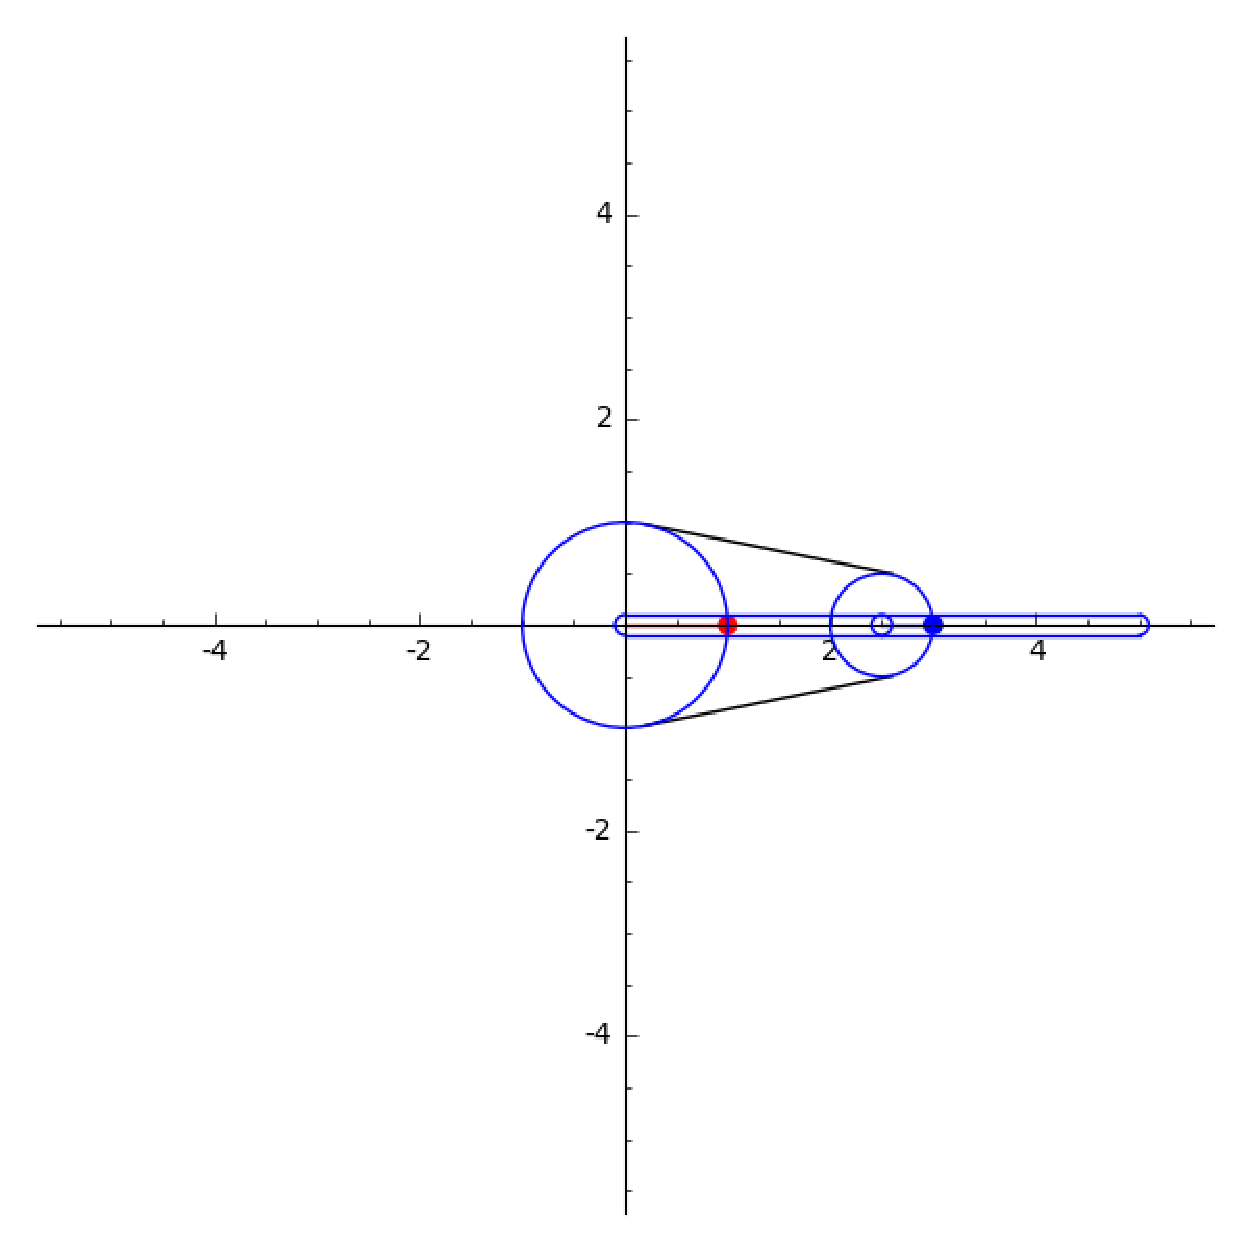
\includegraphics[width=0.25\columnwidth]{tri1.eps}
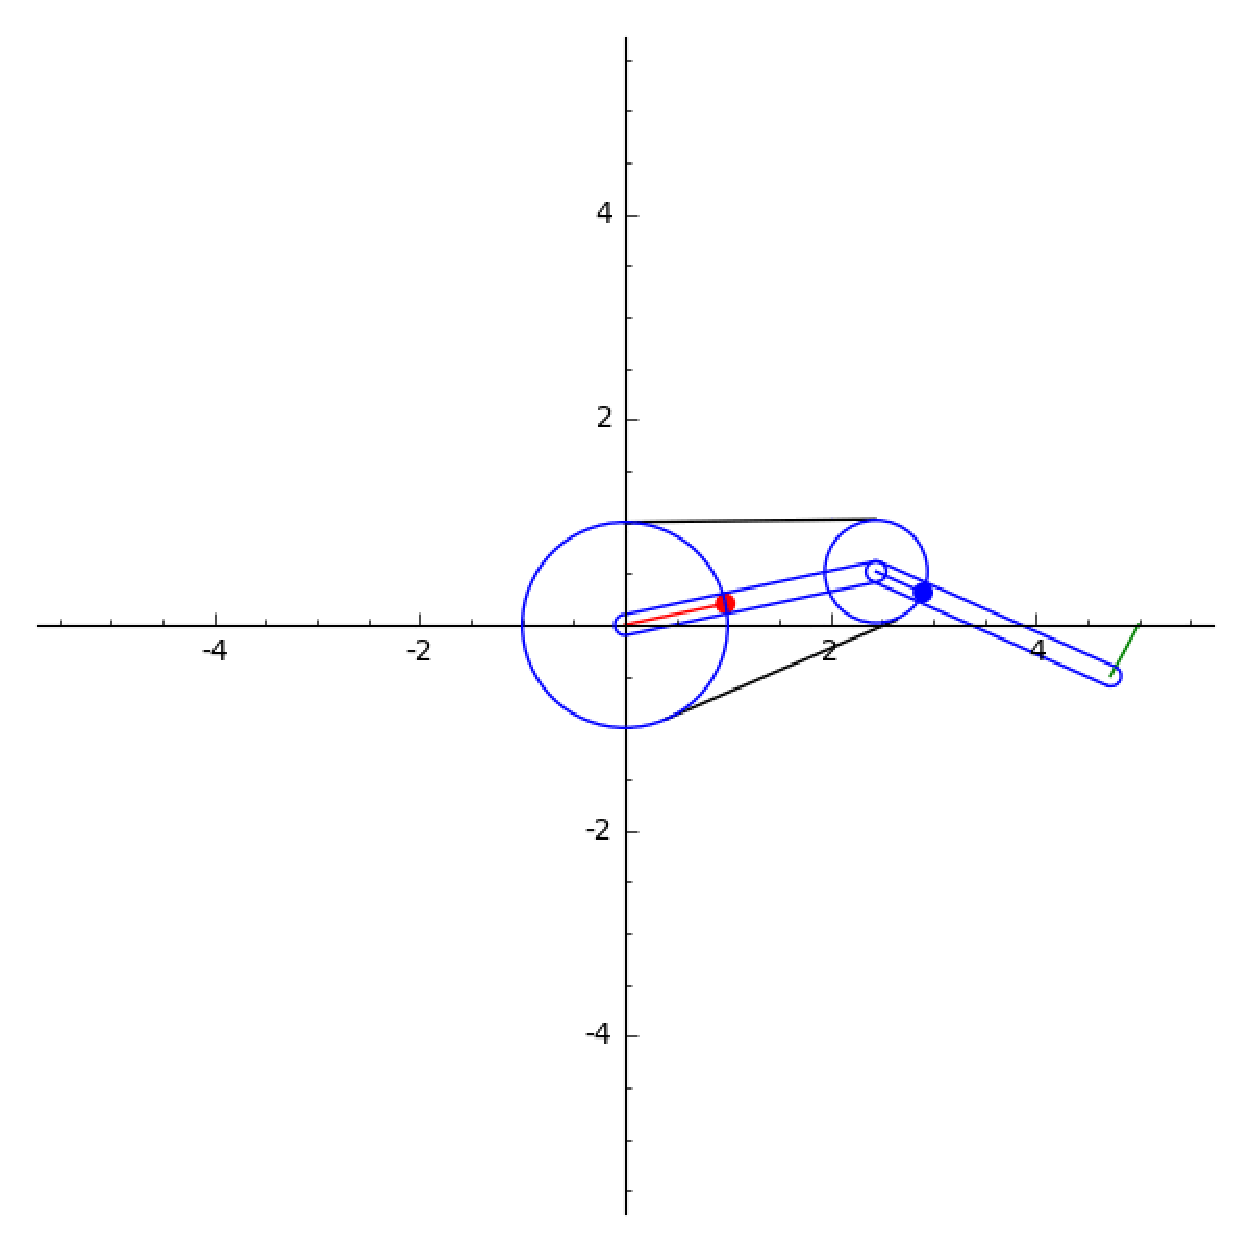
\includegraphics[width=0.25\columnwidth]{tri2.eps}
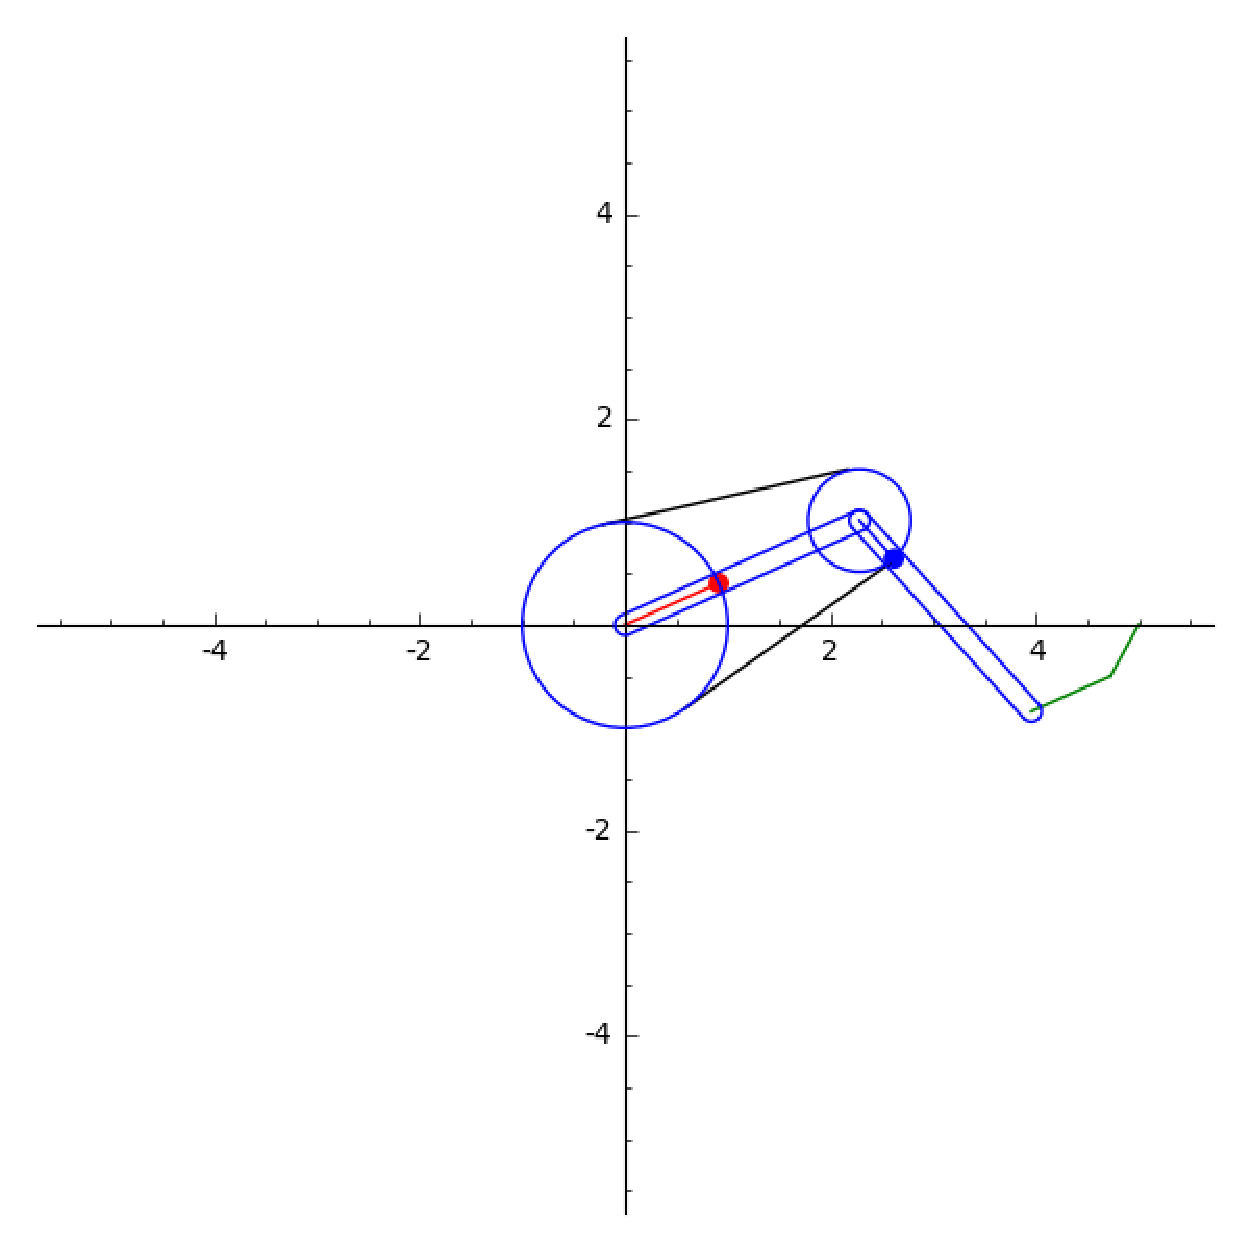
\includegraphics[width=0.25\columnwidth]{tri3.eps}
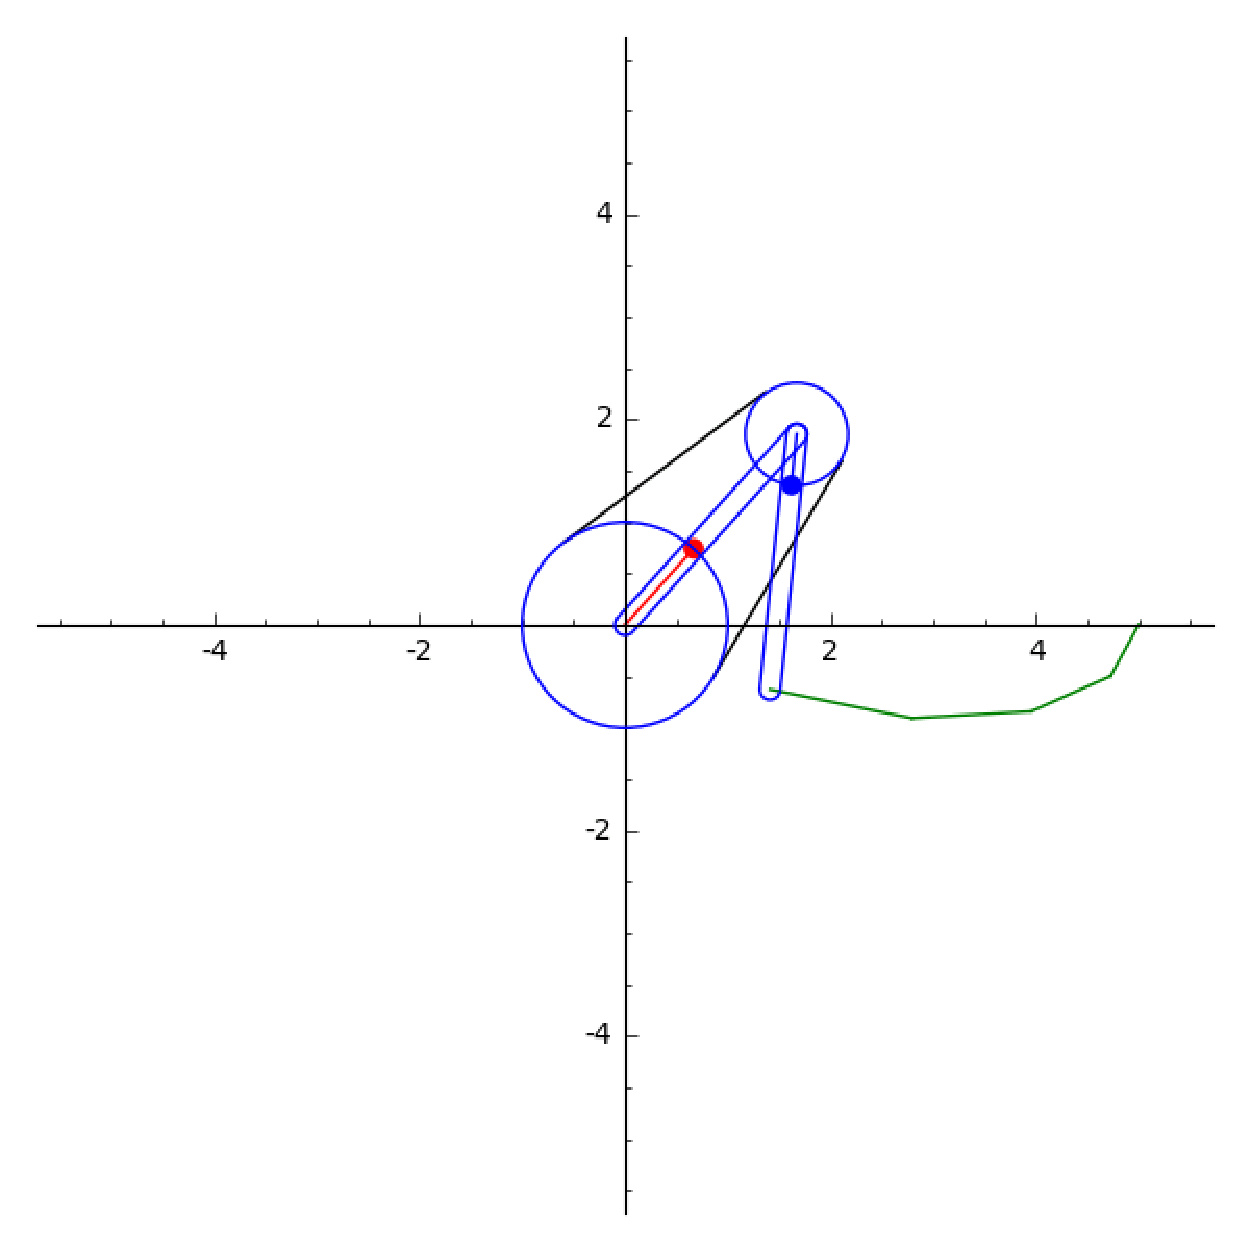
\includegraphics[width=0.25\columnwidth]{tri5.eps}\\[1em]
\vspace{0.5em}
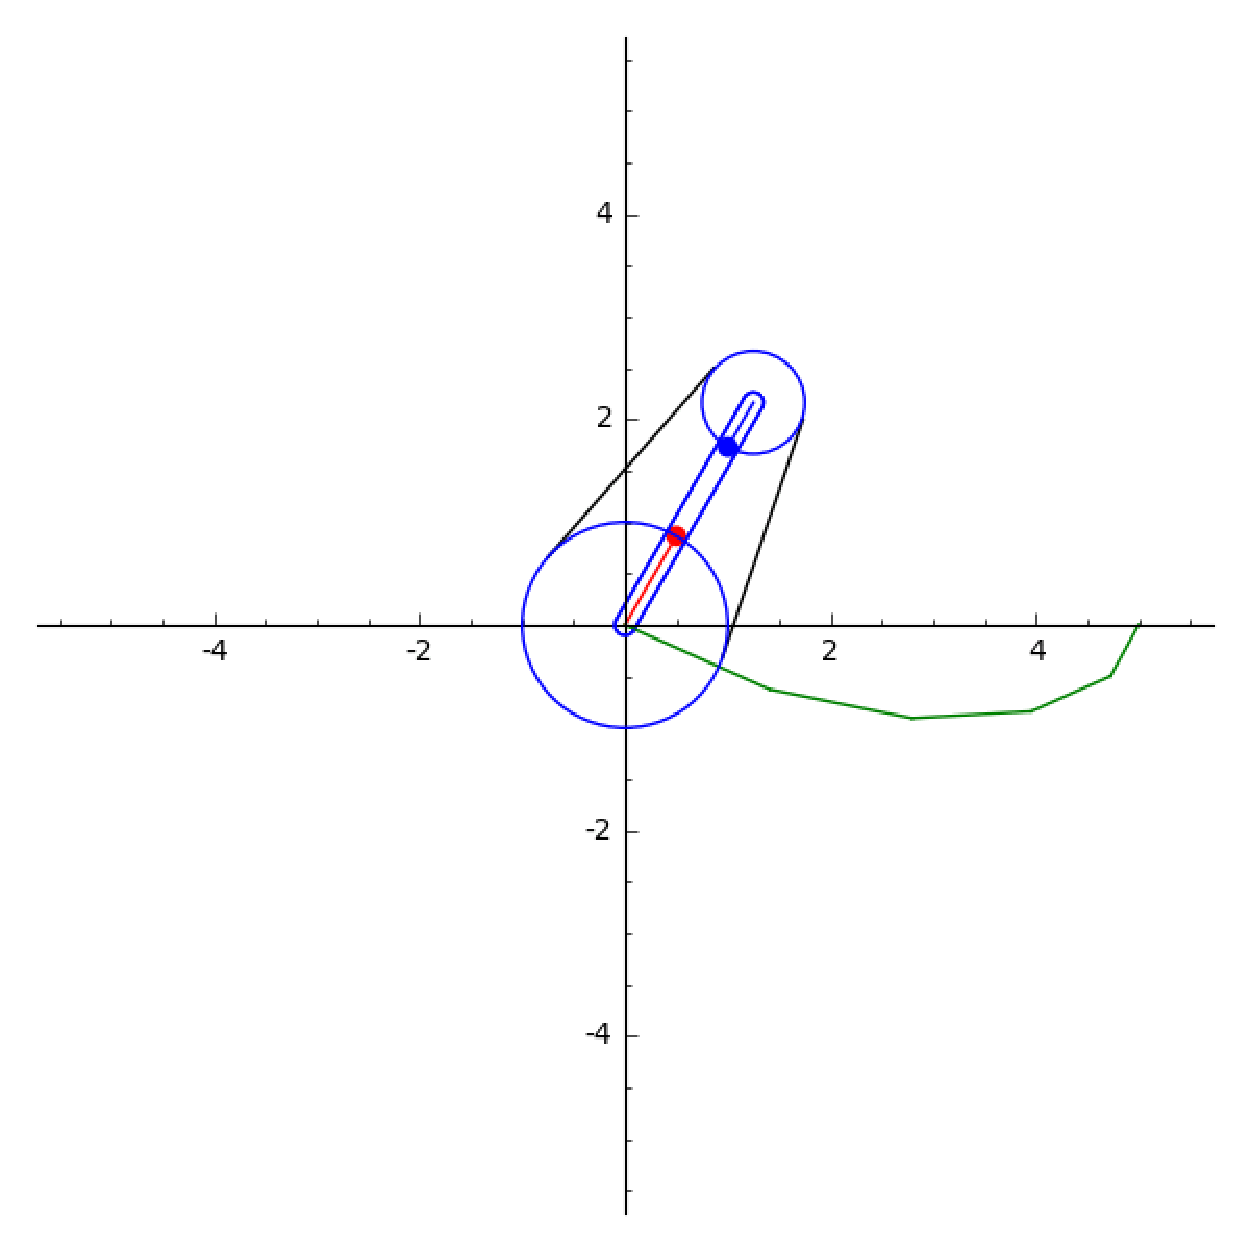
\includegraphics[width=0.25\columnwidth]{tri6.eps}
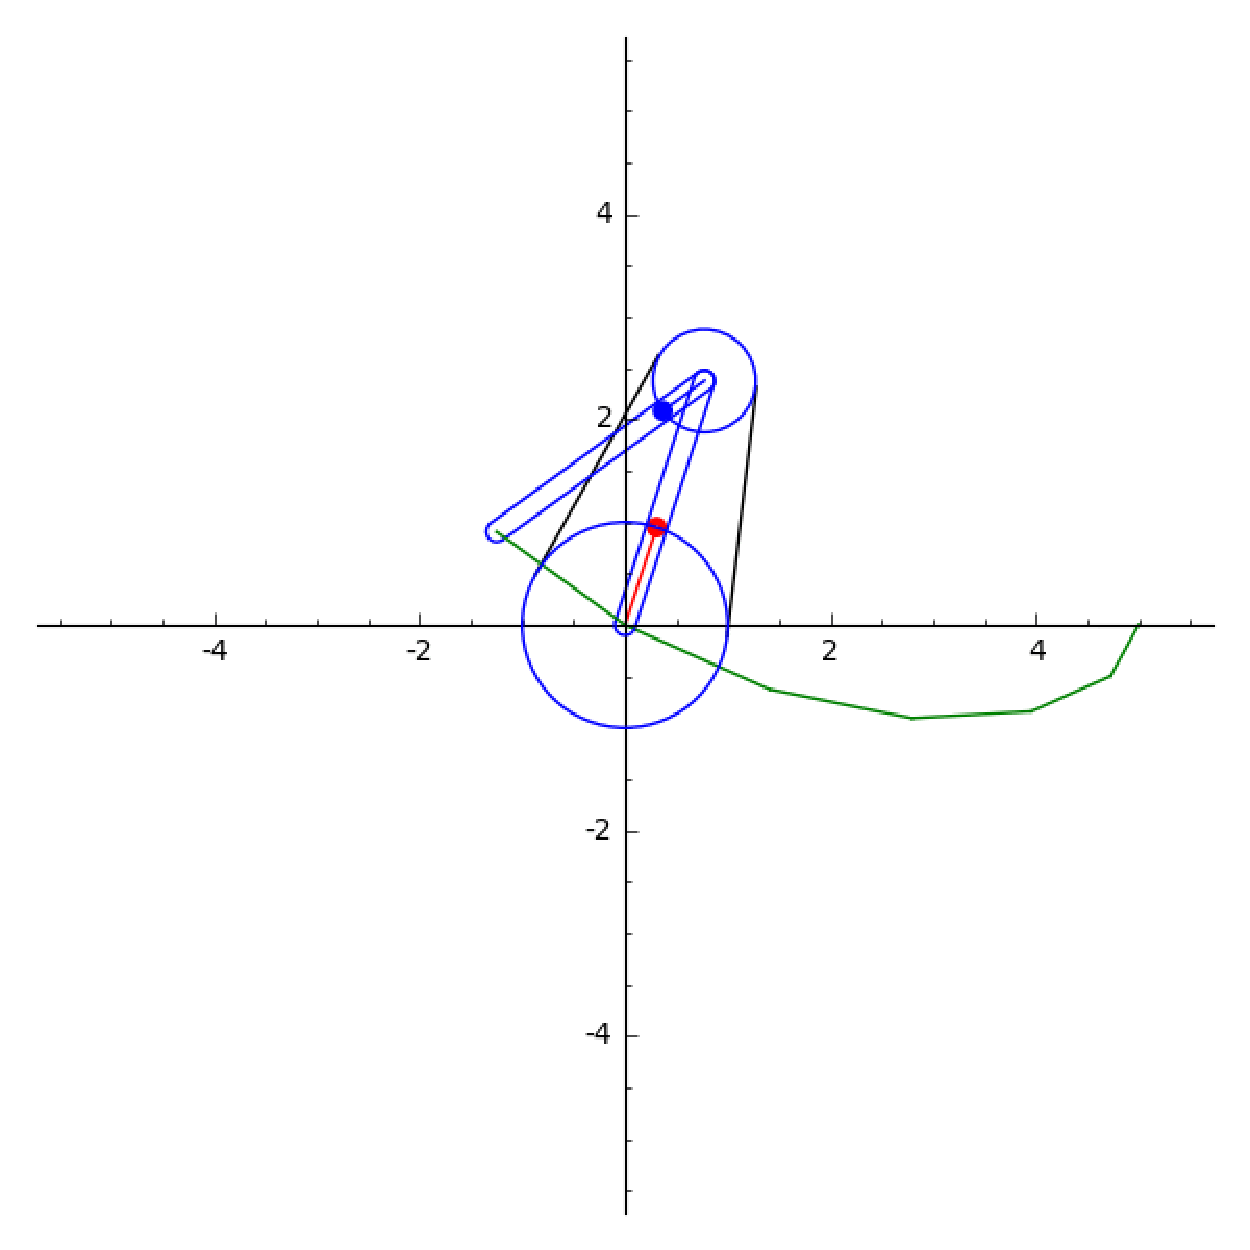
\includegraphics[width=0.25\columnwidth]{tri7.eps}
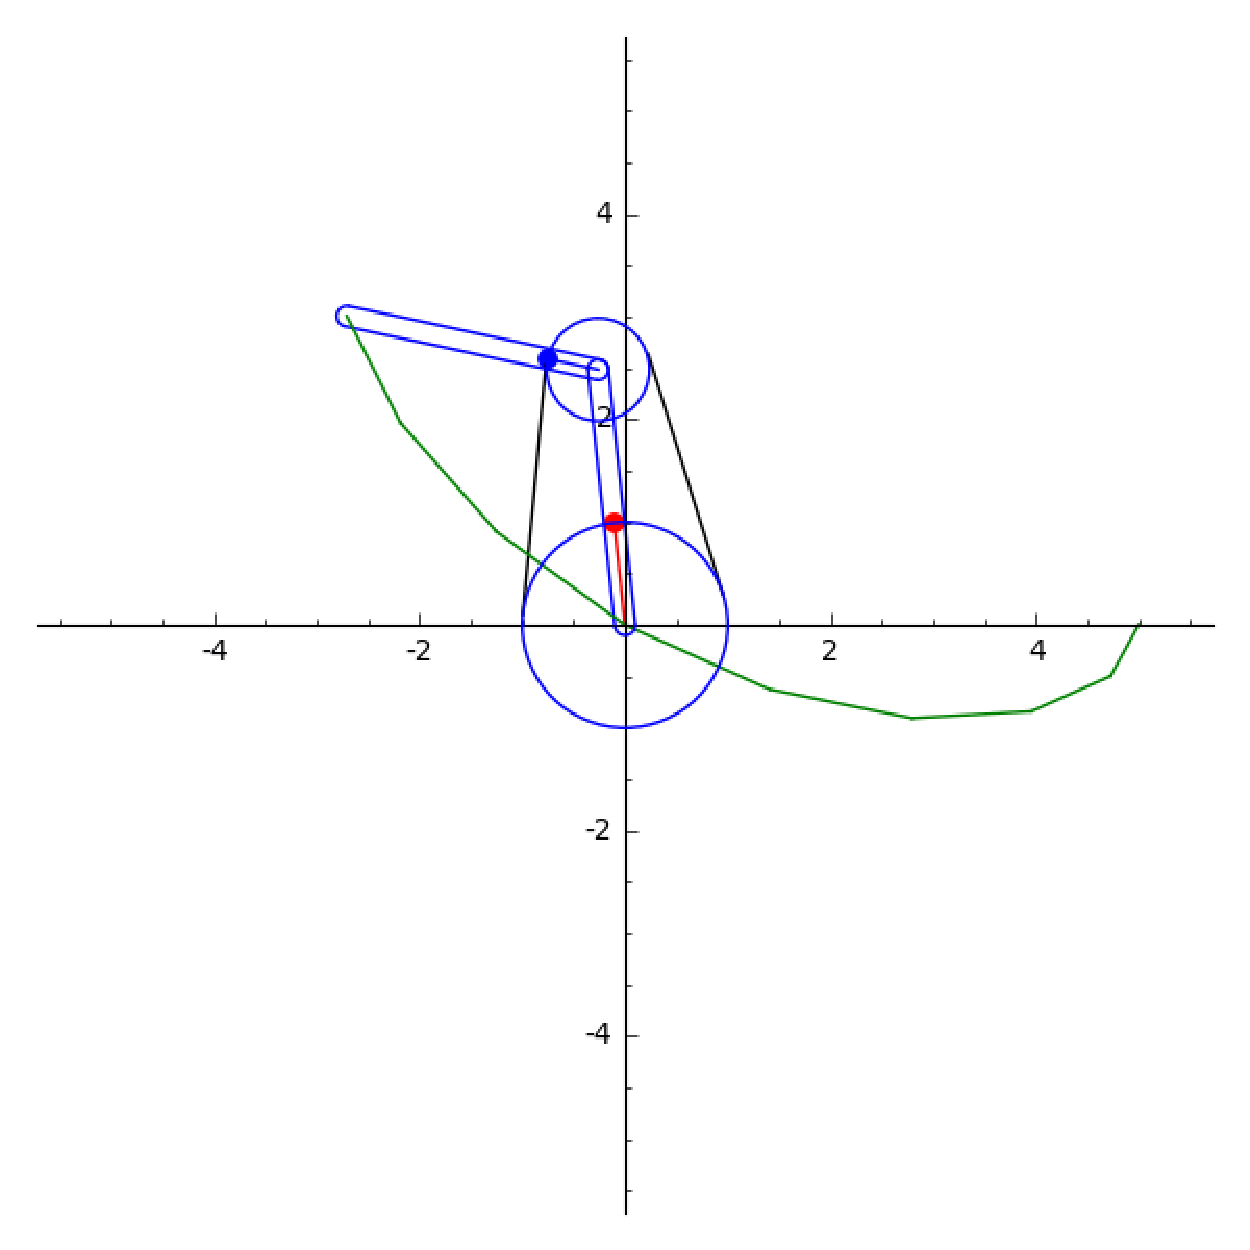
\includegraphics[width=0.25\columnwidth]{tri9.eps}
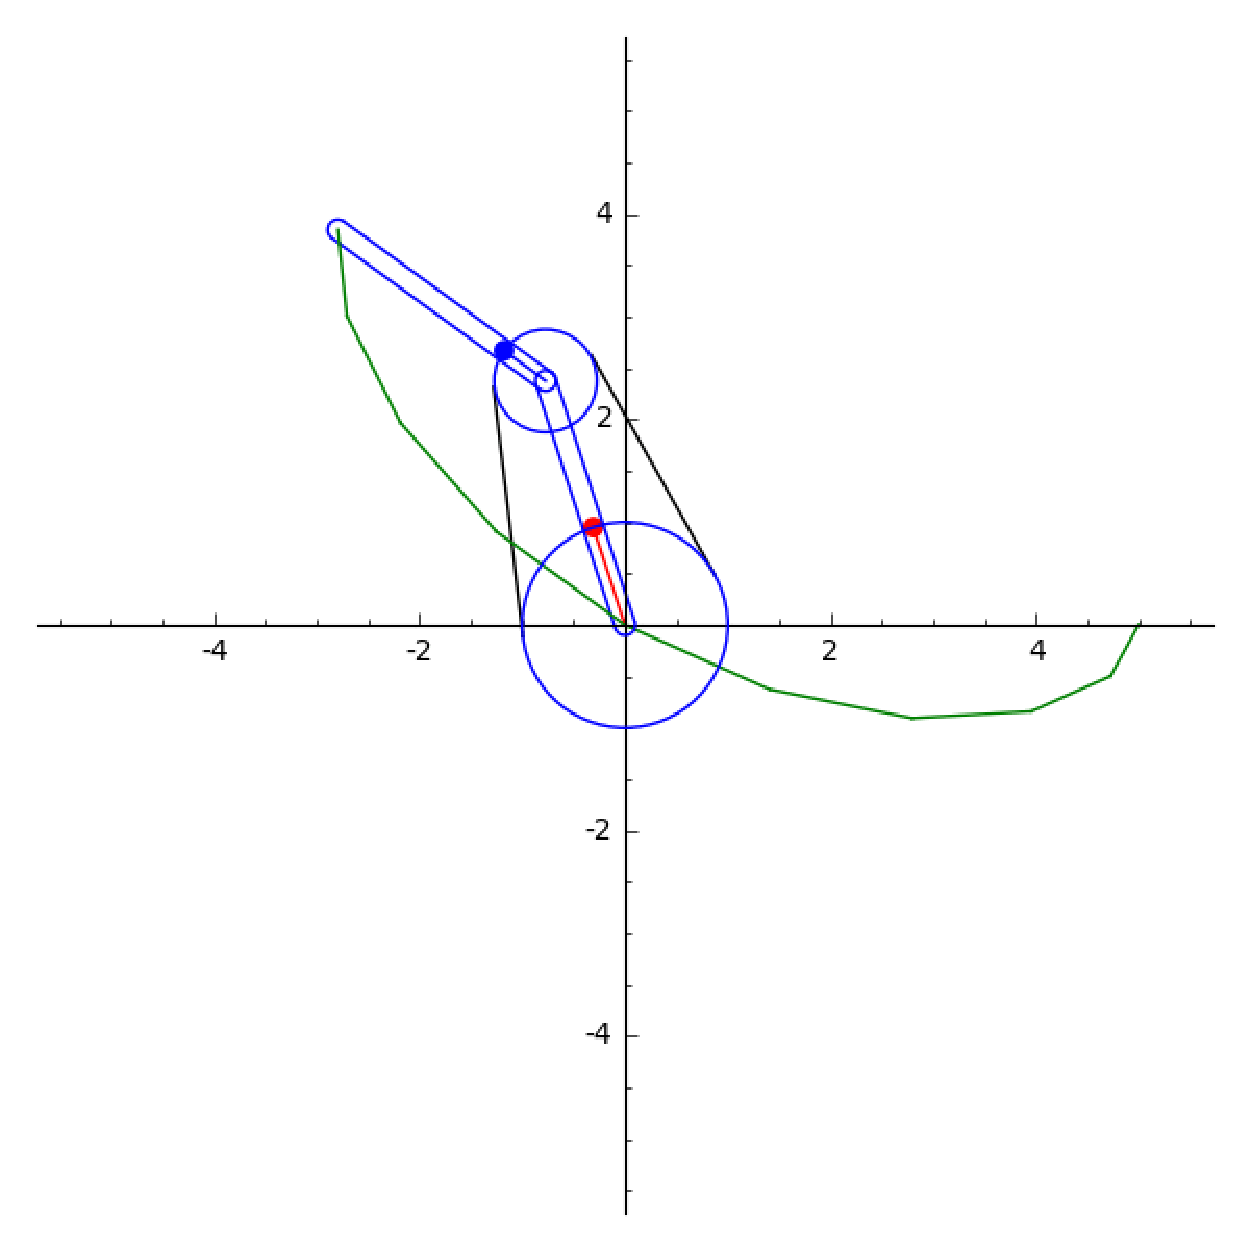
\includegraphics[width=0.25\columnwidth]{tri10.eps}\\[1em]
\vspace{1em}
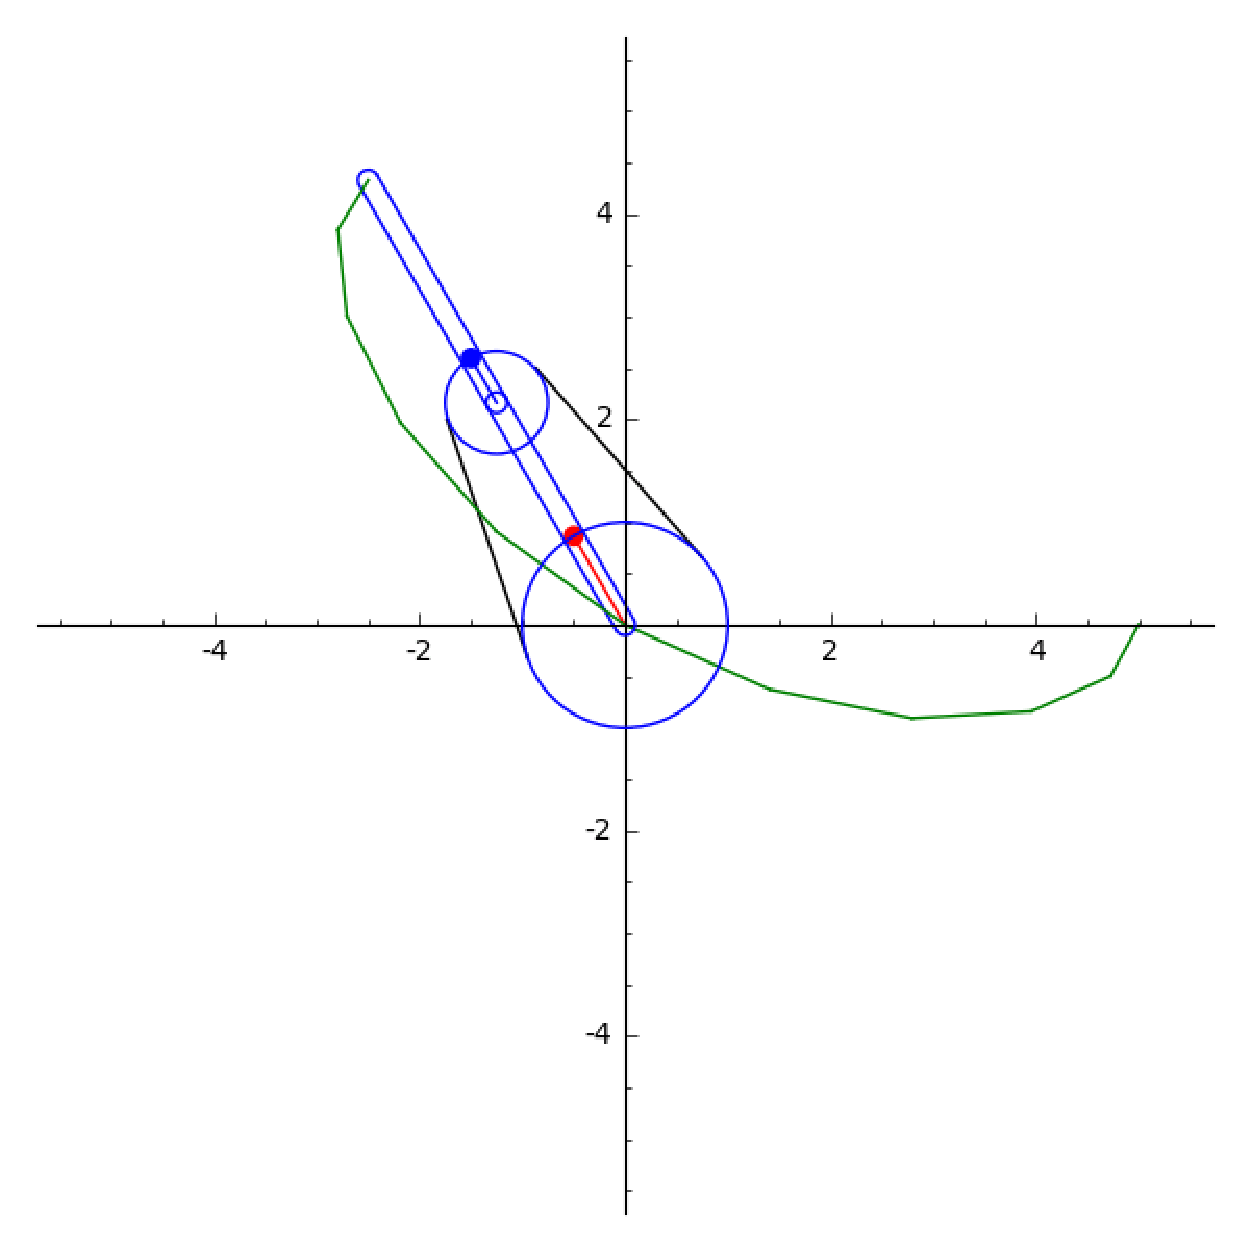
\includegraphics[width=0.25\columnwidth]{tri11.eps}
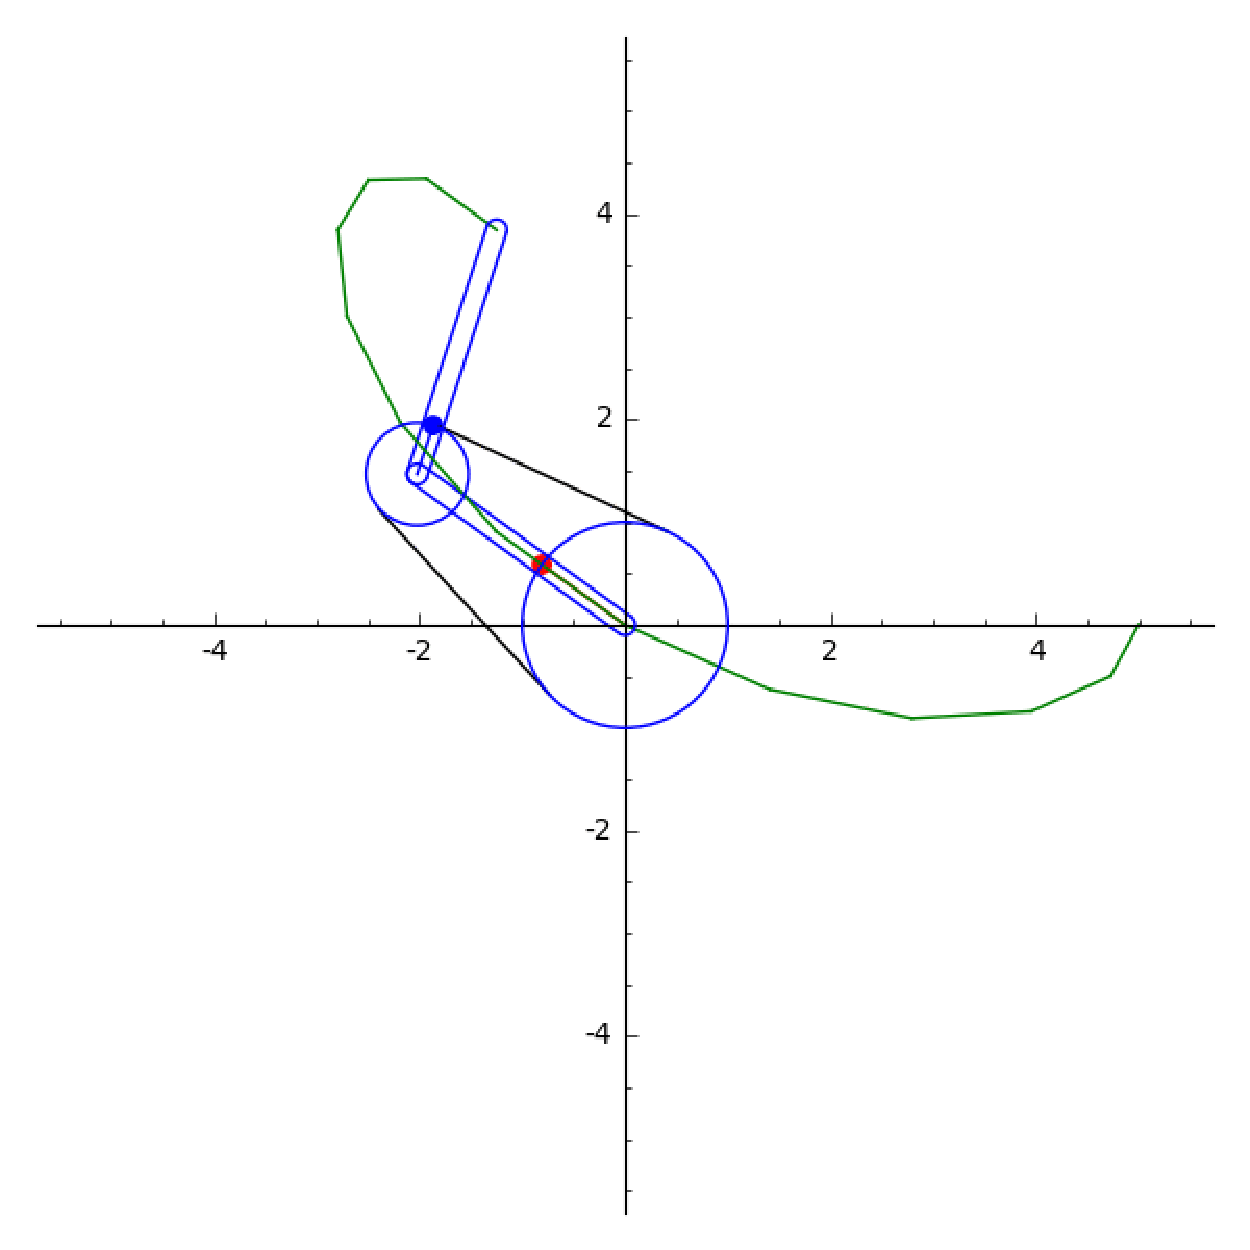
\includegraphics[width=0.25\columnwidth]{tri13.eps}
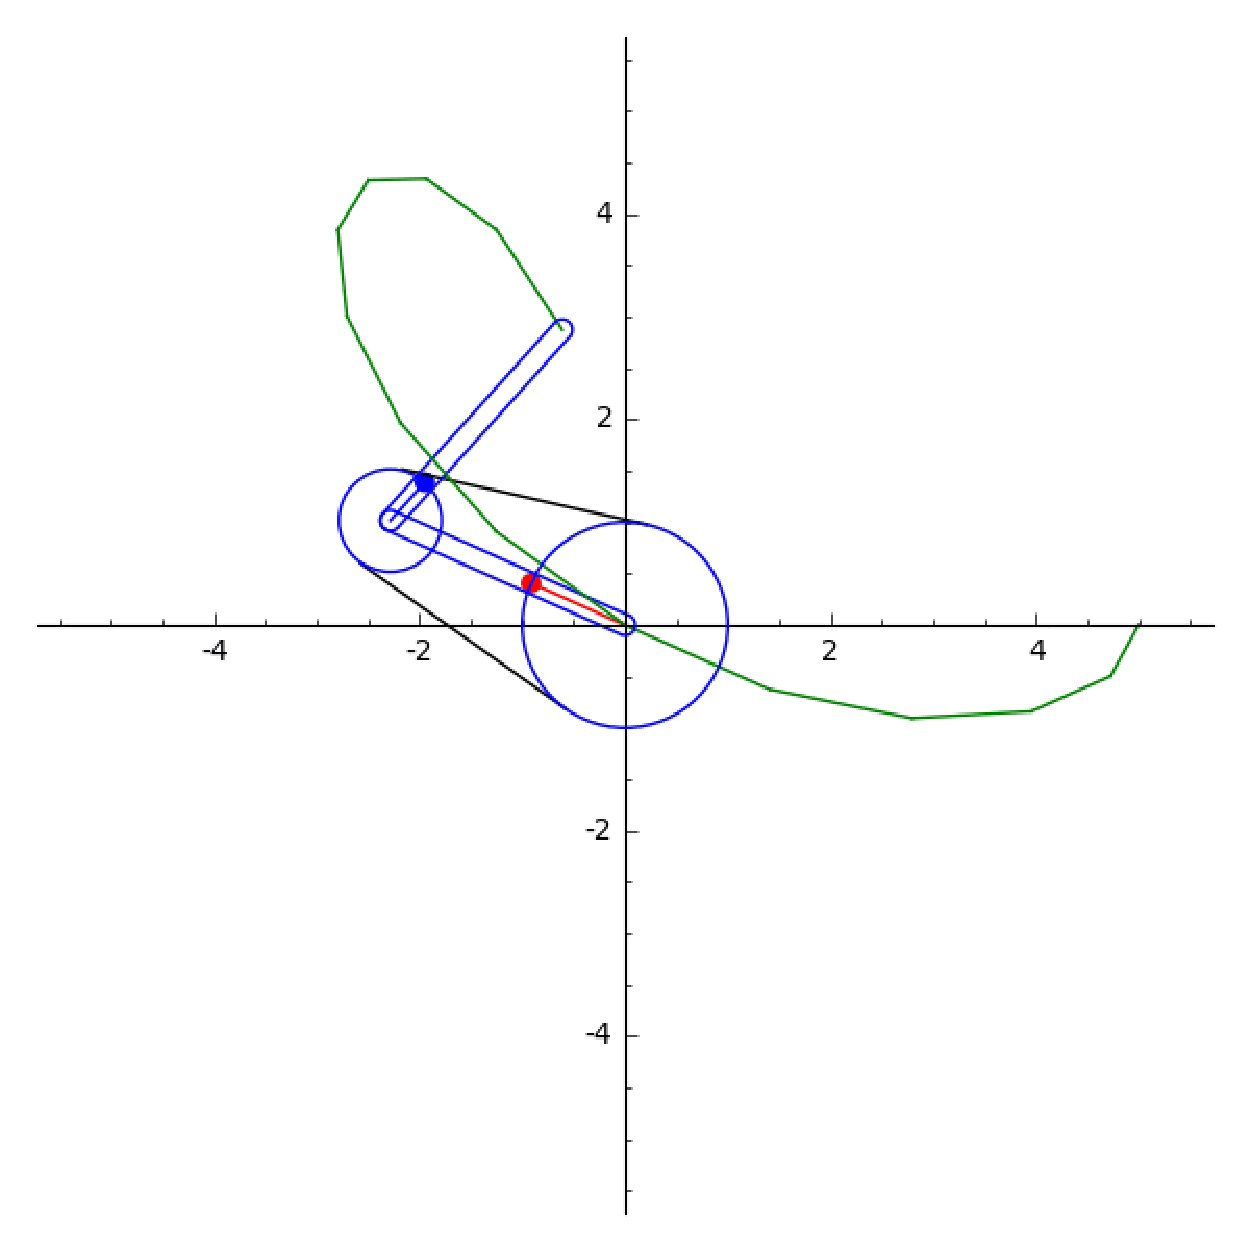
\includegraphics[width=0.25\columnwidth]{tri14.eps}
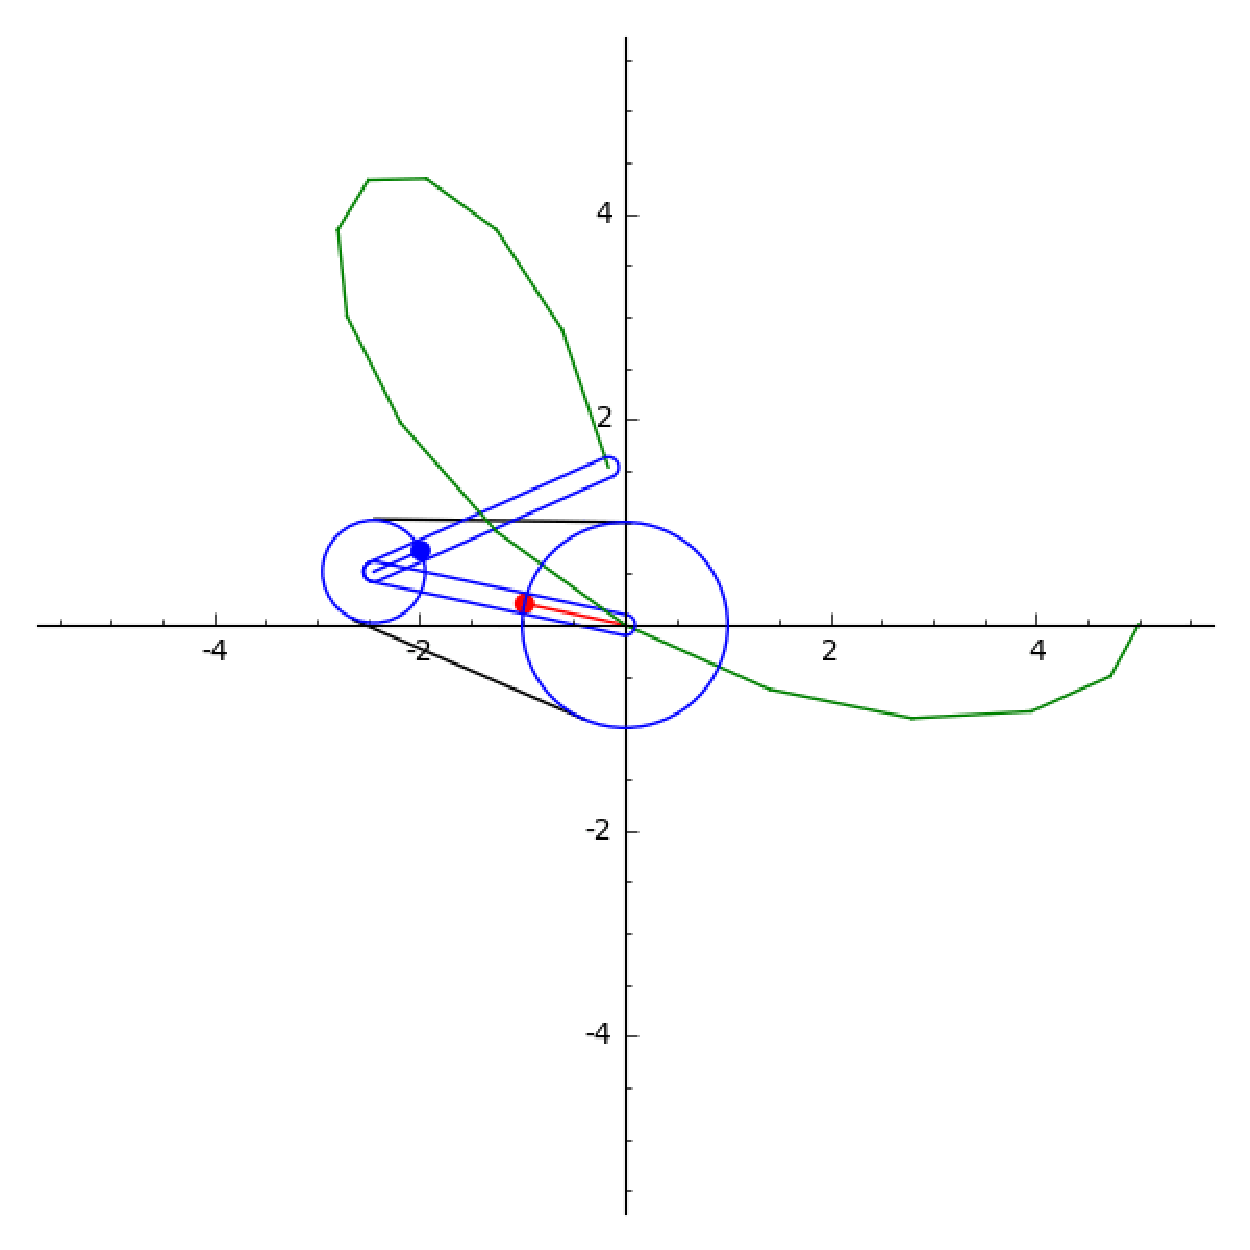
\includegraphics[width=0.25\columnwidth]{tri15.eps}\\[1em]
\vspace{1em}
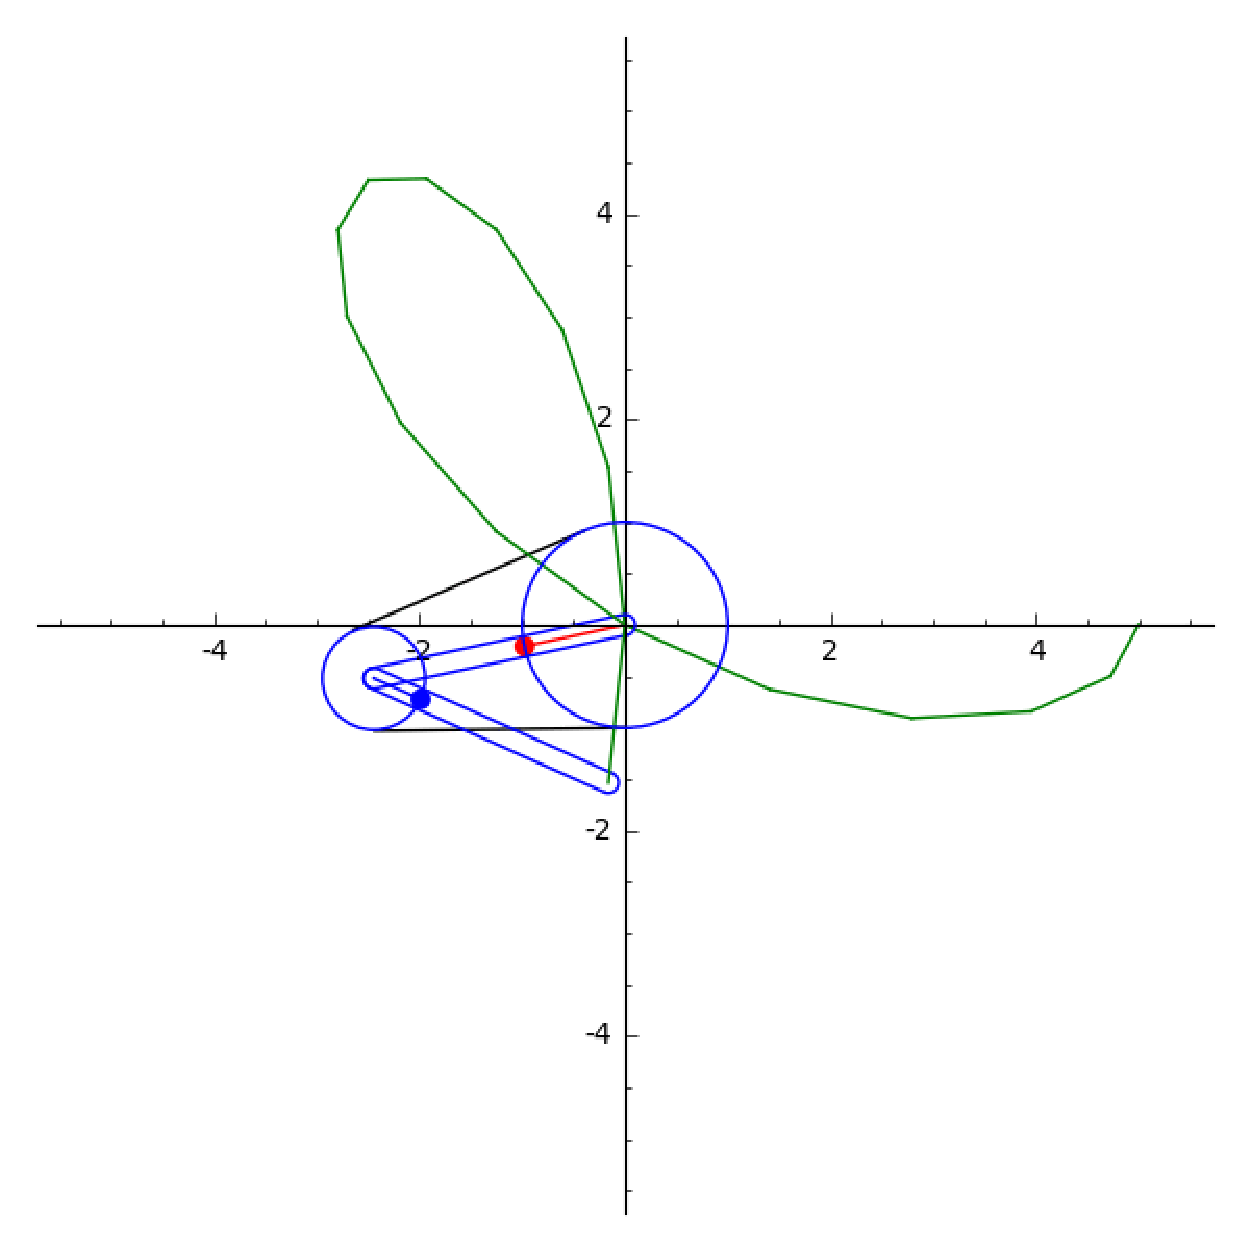
\includegraphics[width=0.25\columnwidth]{tri17.eps}
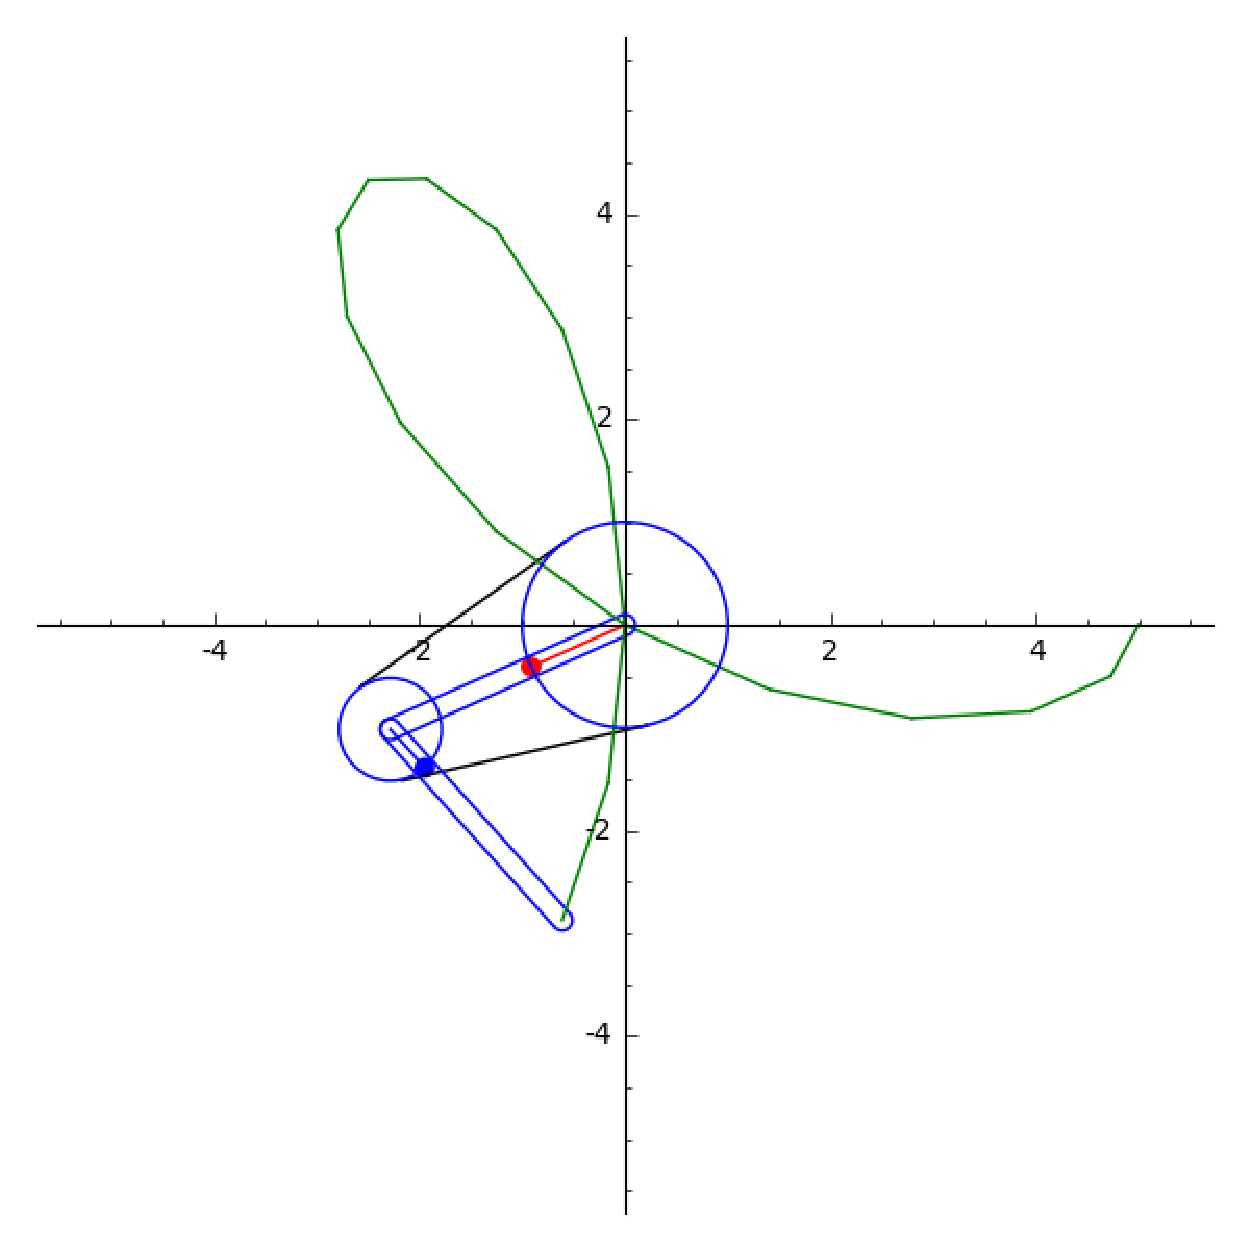
\includegraphics[width=0.25\columnwidth]{tri18.eps}
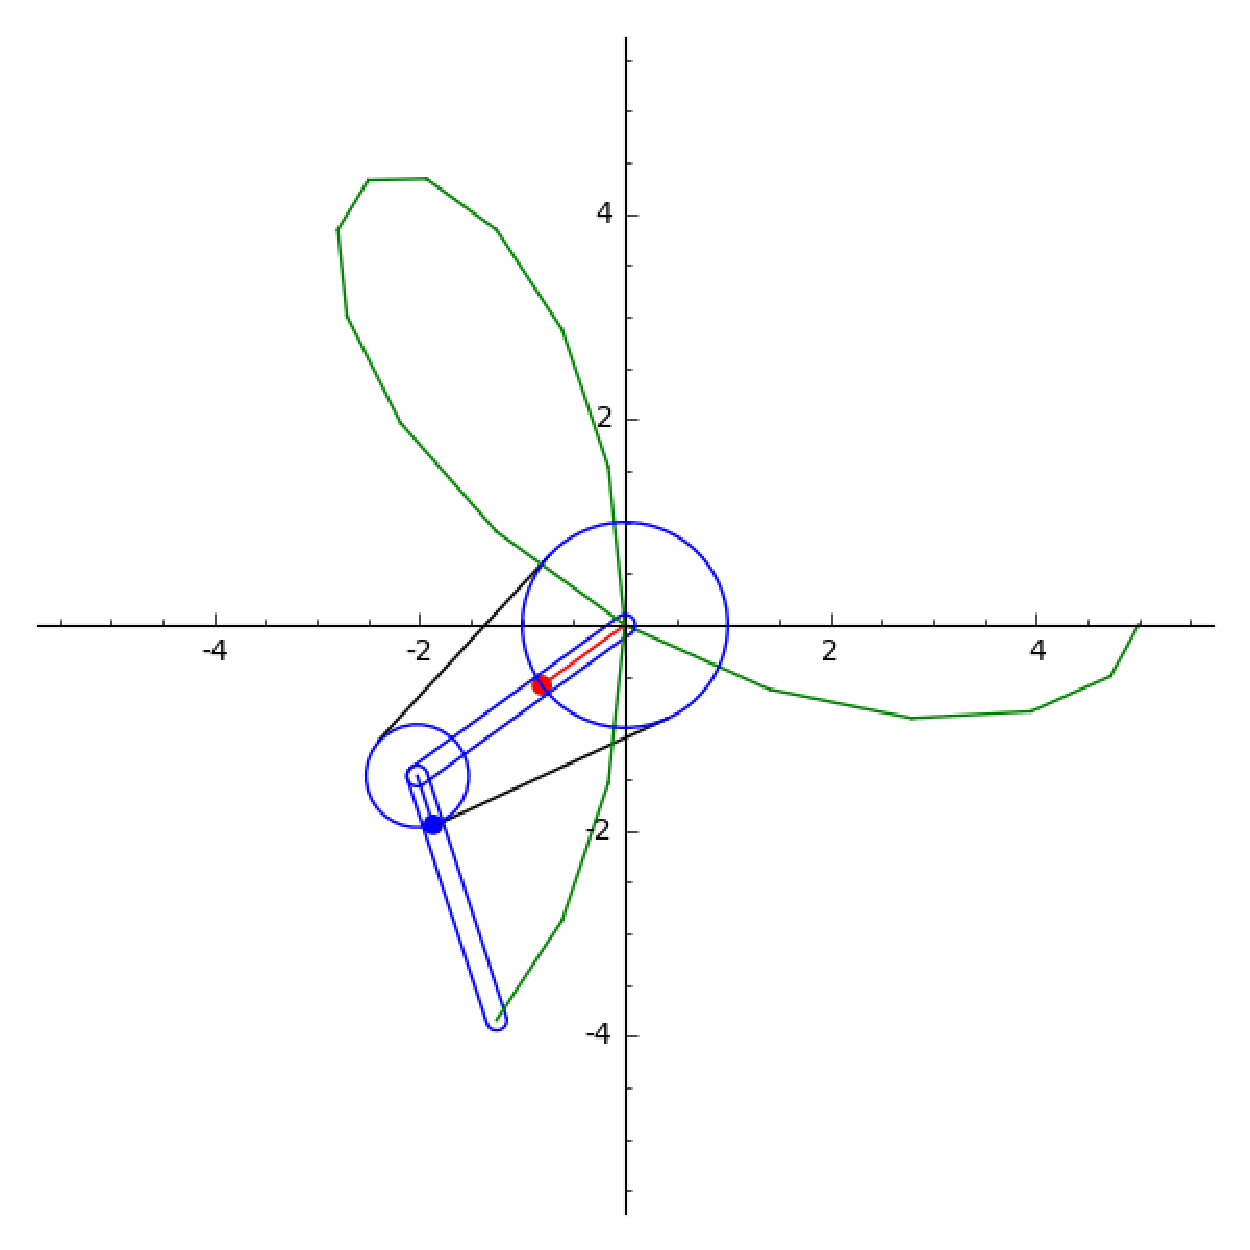
\includegraphics[width=0.25\columnwidth]{tri19.eps}
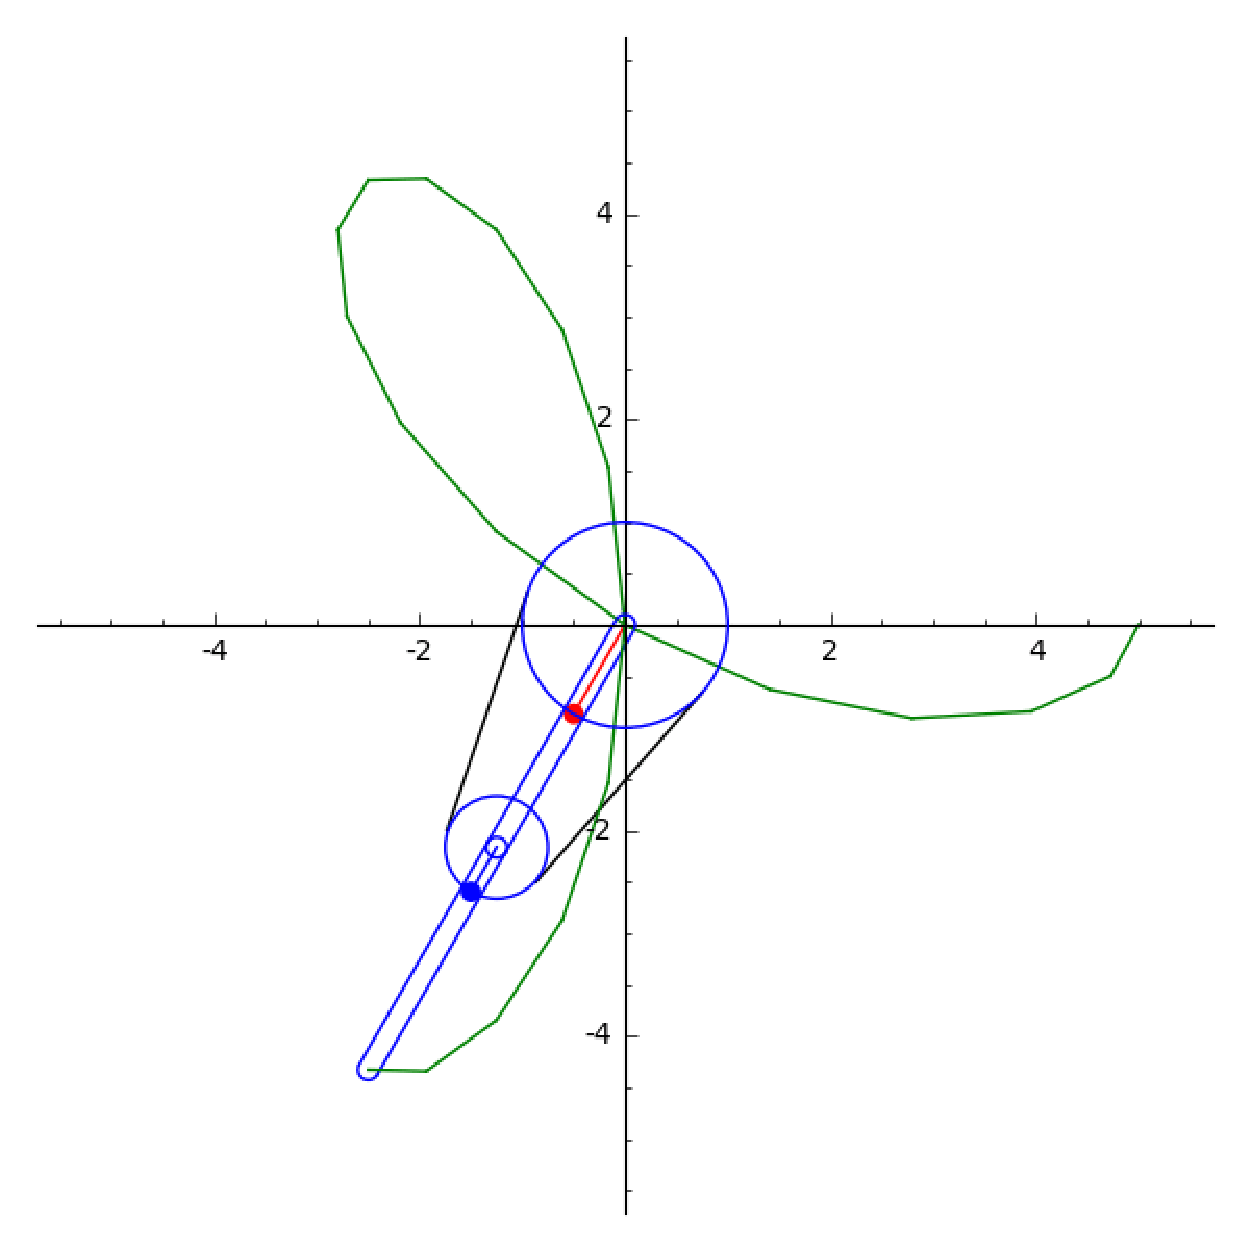
\includegraphics[width=0.25\columnwidth]{tri21.eps}\\[1em]
\vspace{1em}
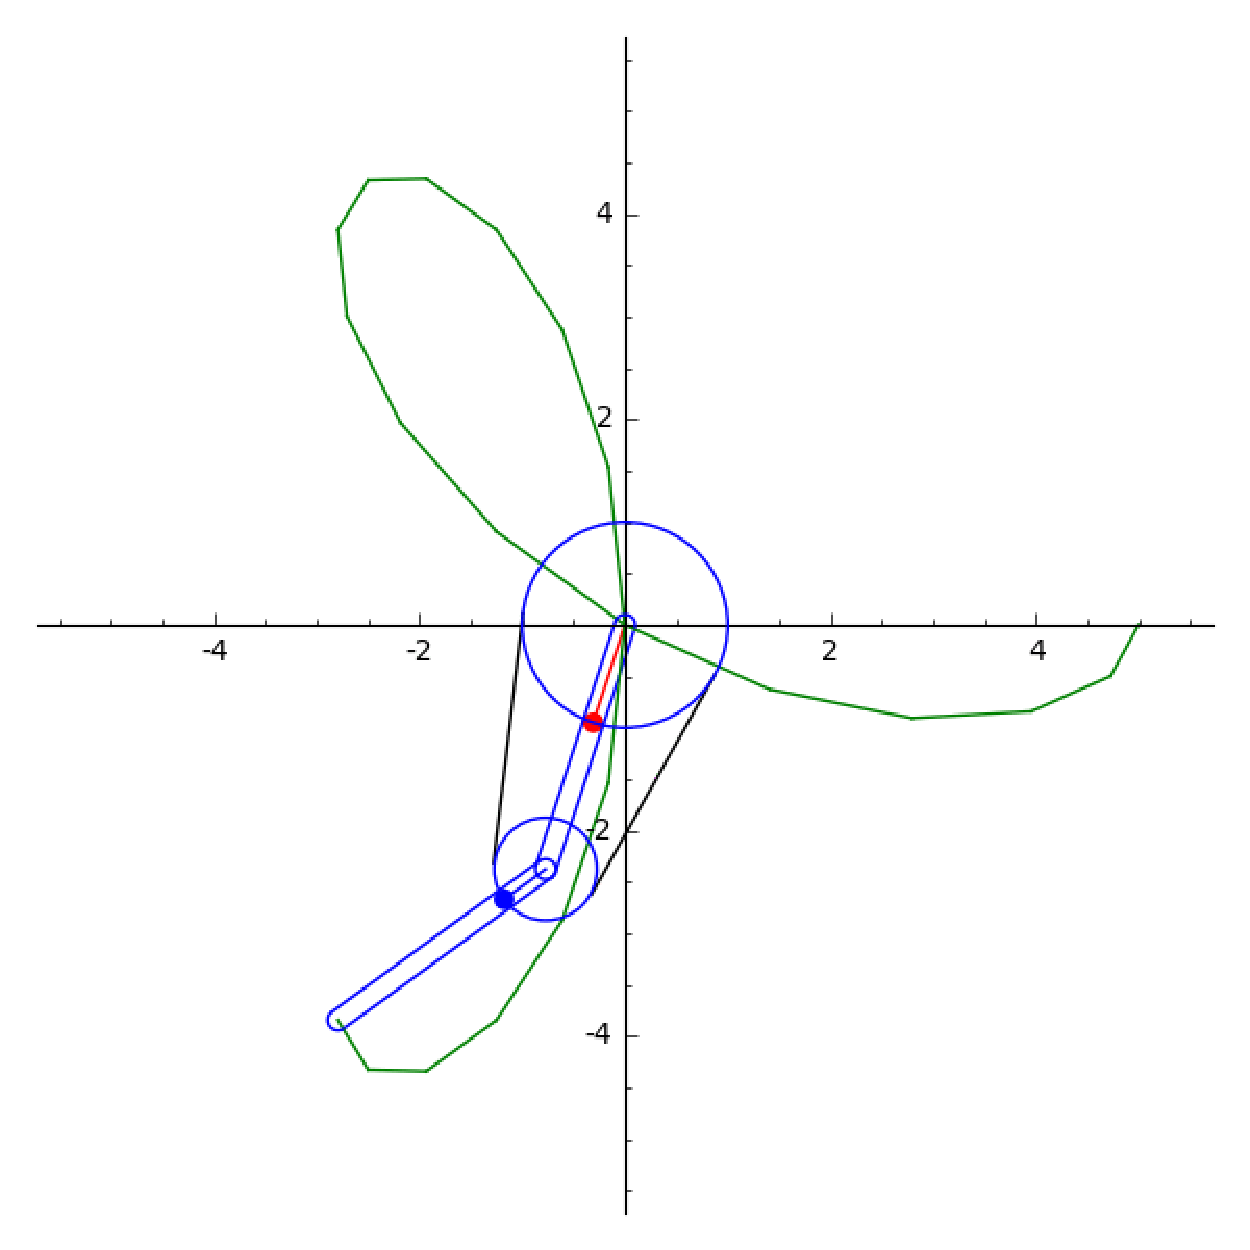
\includegraphics[width=0.25\columnwidth]{tri22.eps}
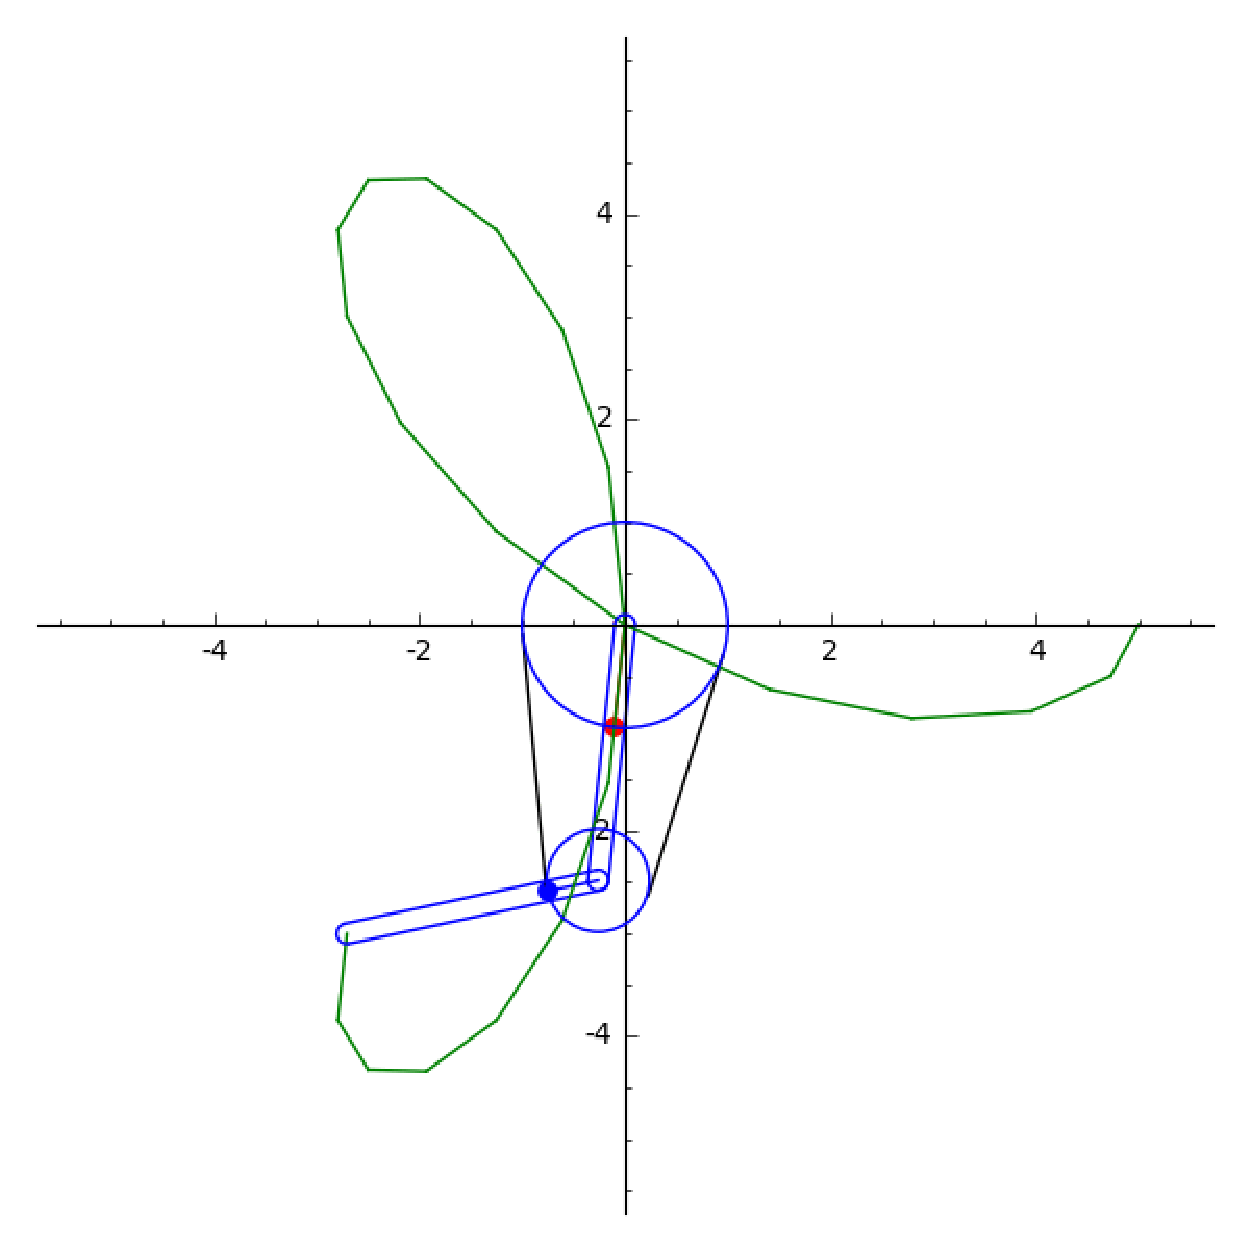
\includegraphics[width=0.25\columnwidth]{tri23.eps}
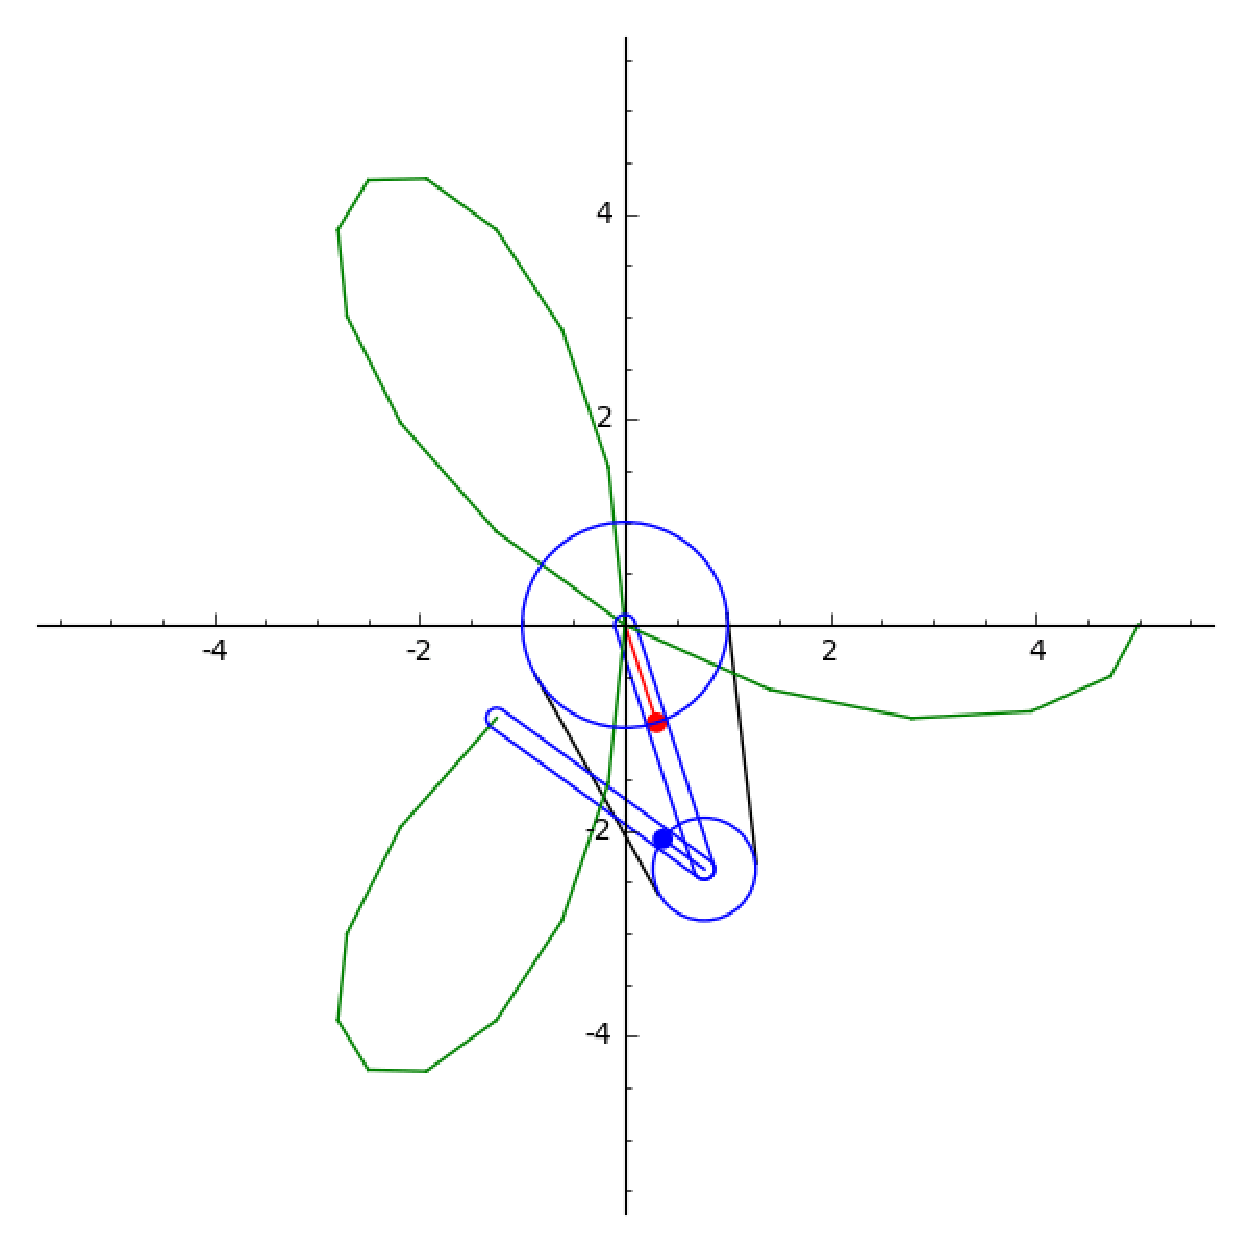
\includegraphics[width=0.25\columnwidth]{tri25.eps}
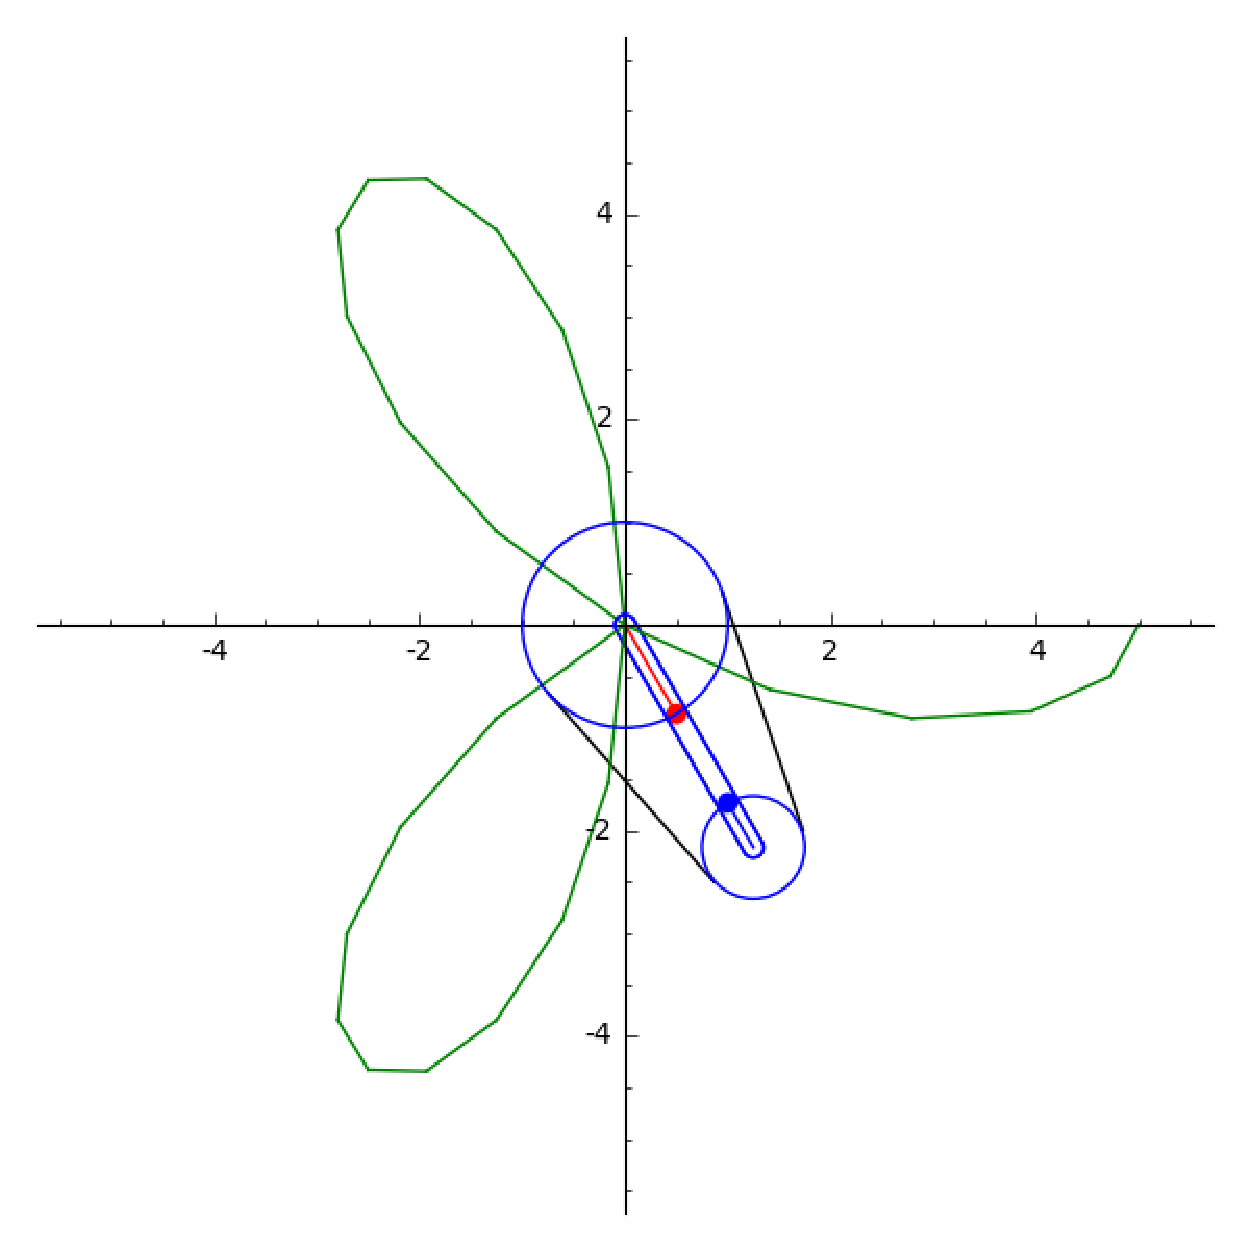
\includegraphics[width=0.25\columnwidth]{tri26.eps}\\[1em]
\vspace{1em}
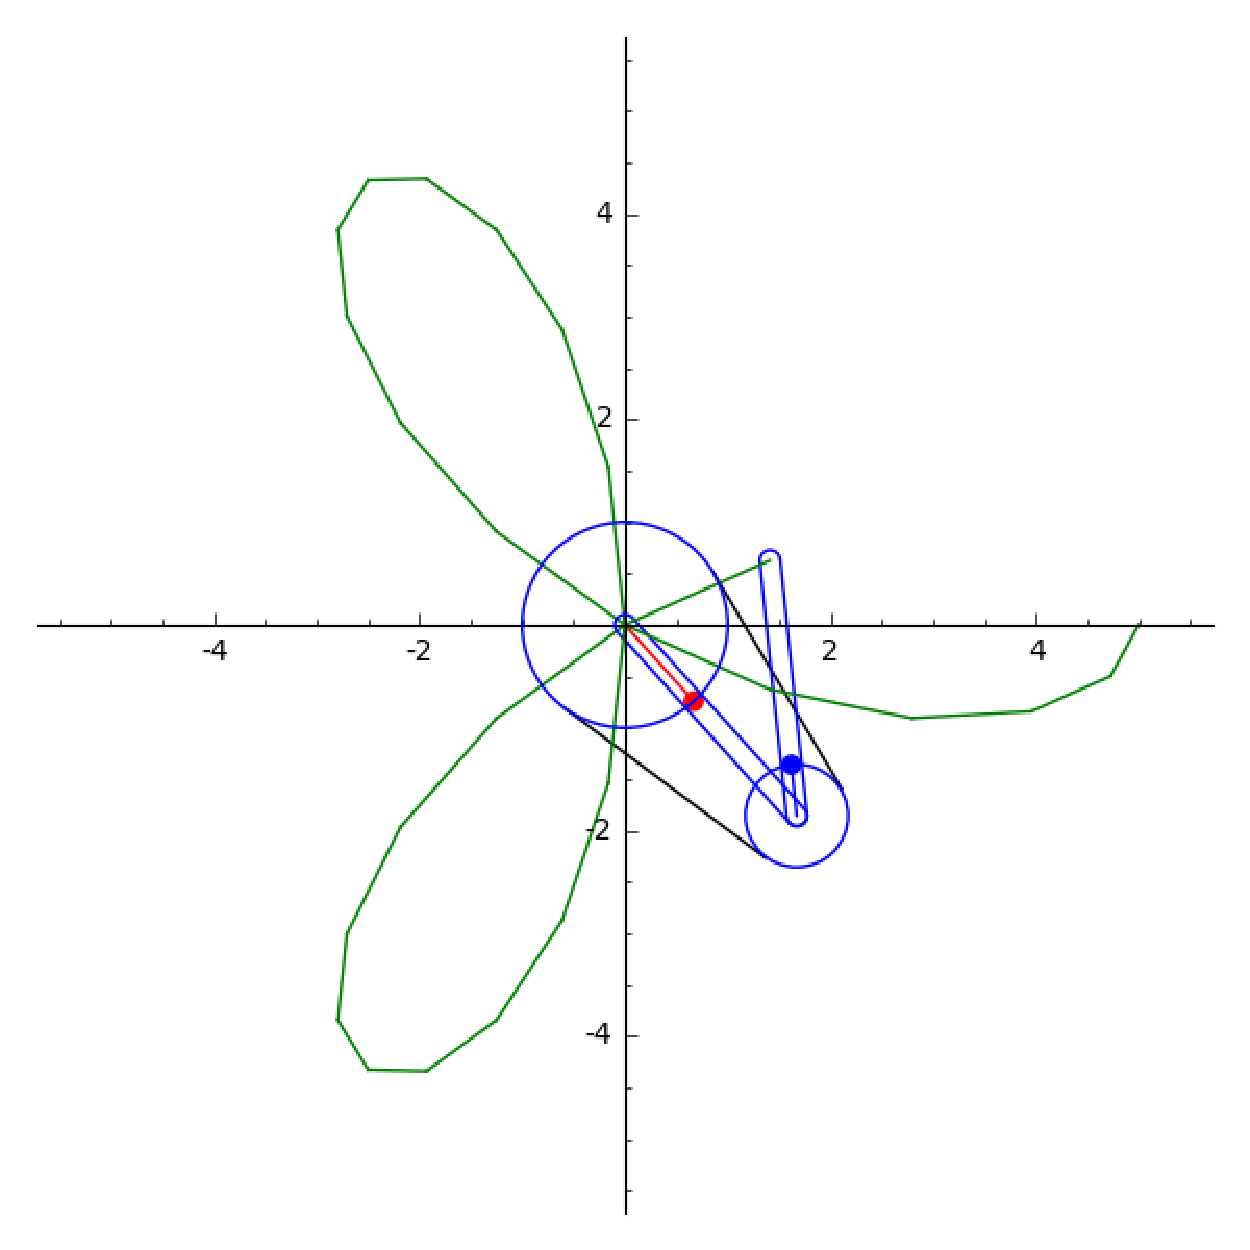
\includegraphics[width=0.25\columnwidth]{tri27.eps}
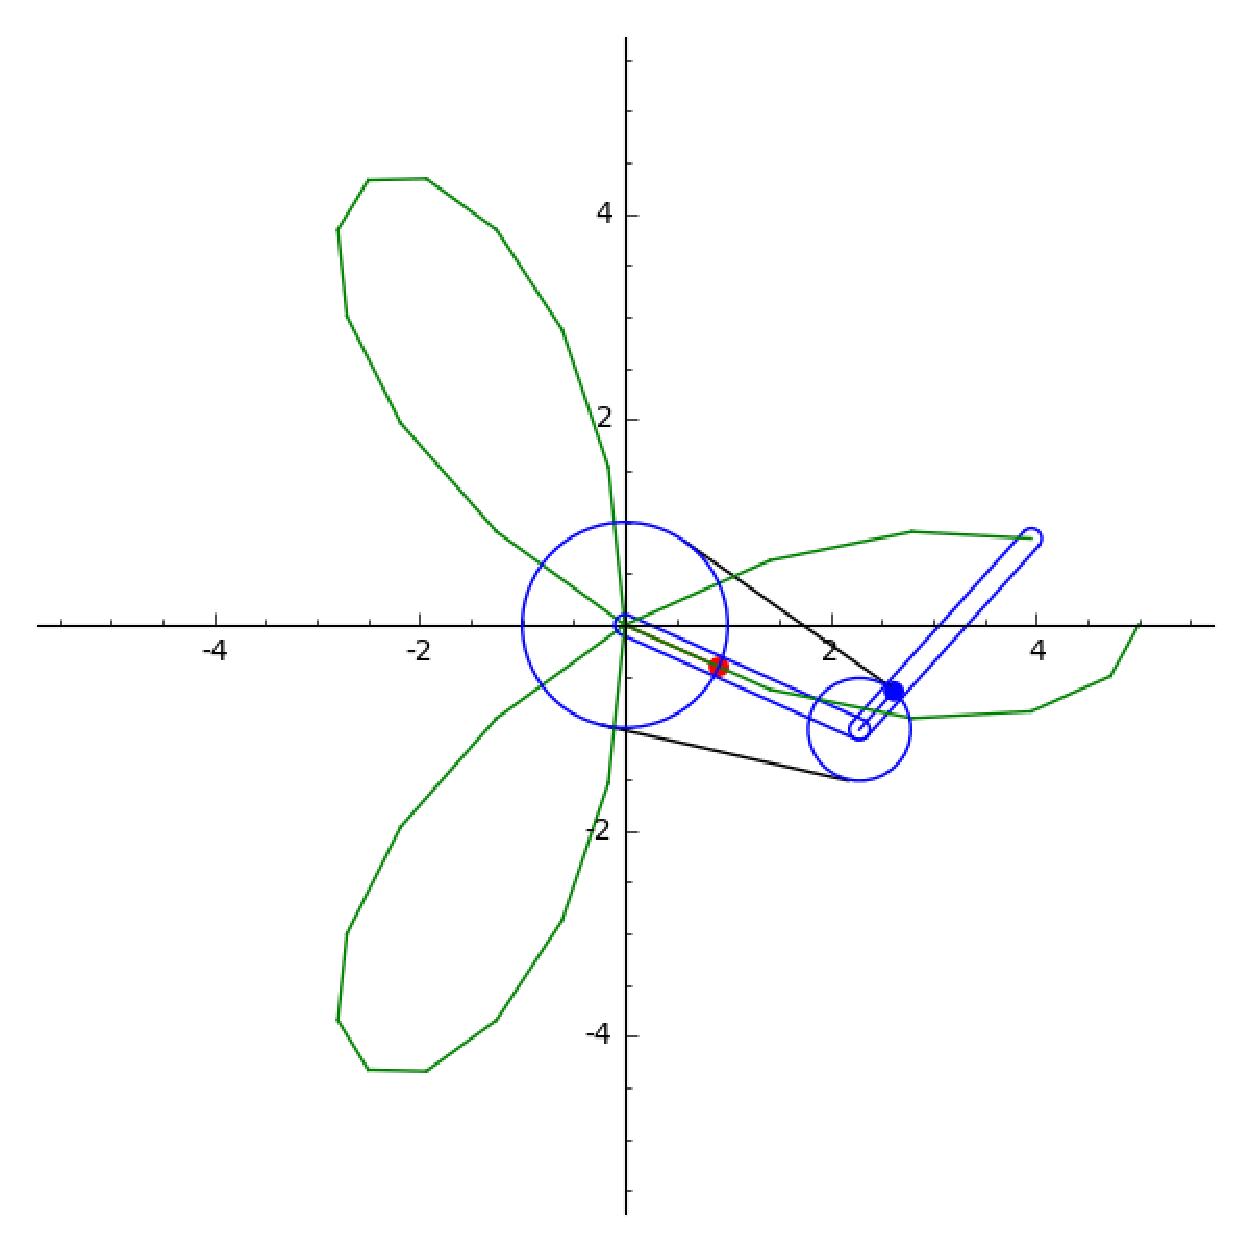
\includegraphics[width=0.25\columnwidth]{tri29.eps}
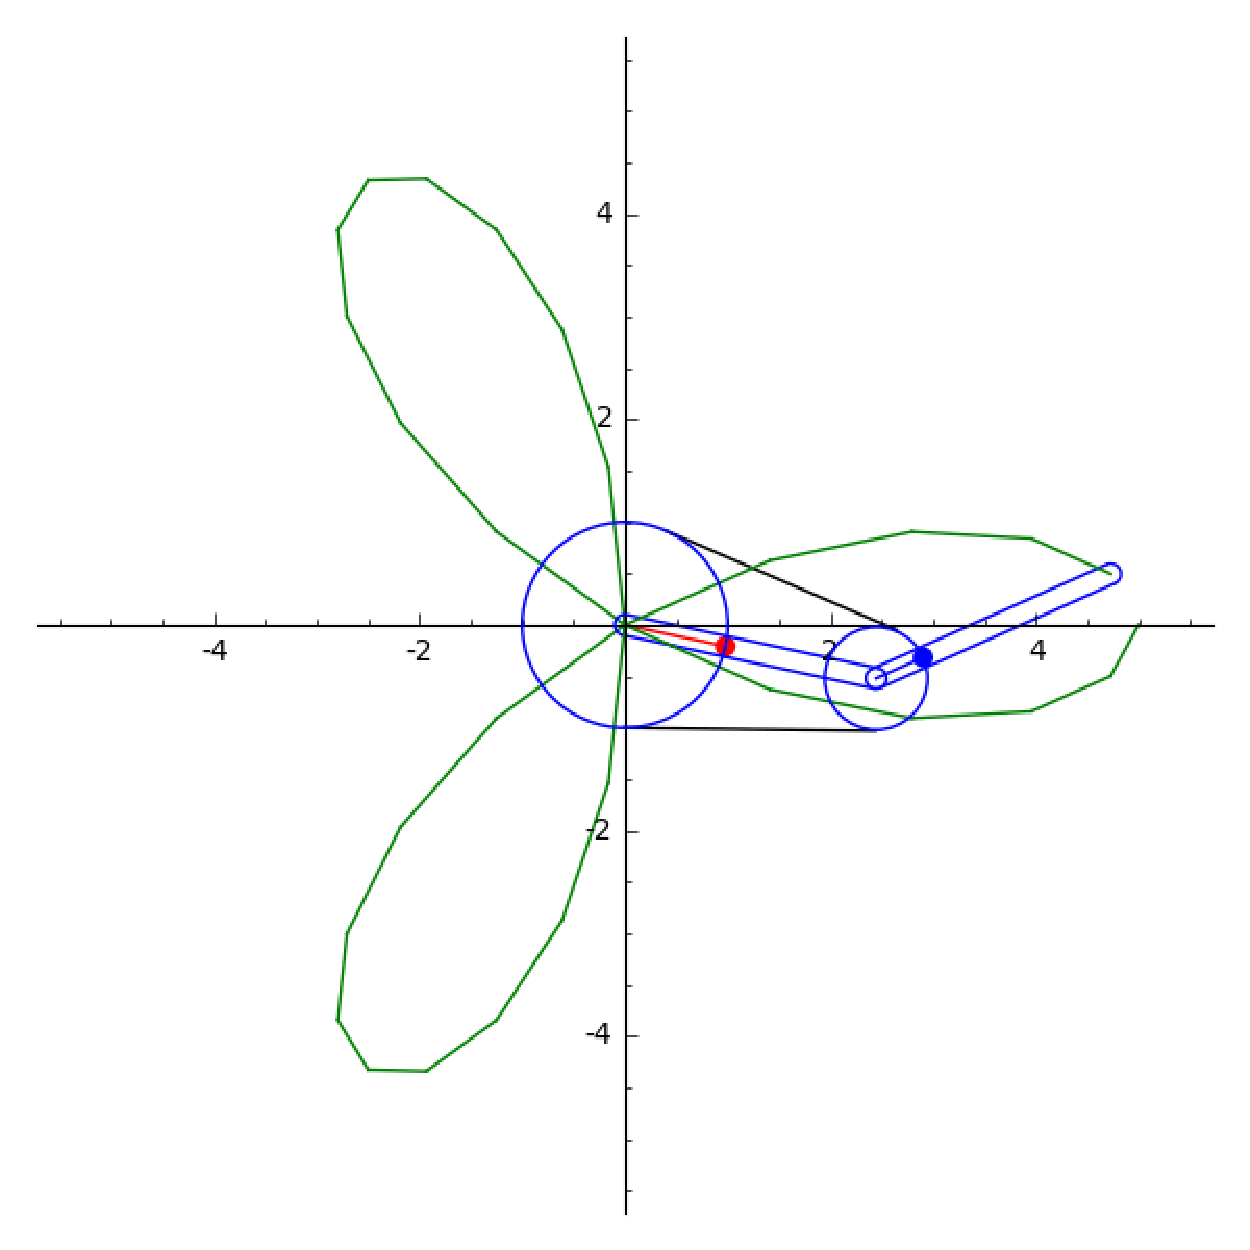
\includegraphics[width=0.25\columnwidth]{tri30.eps}
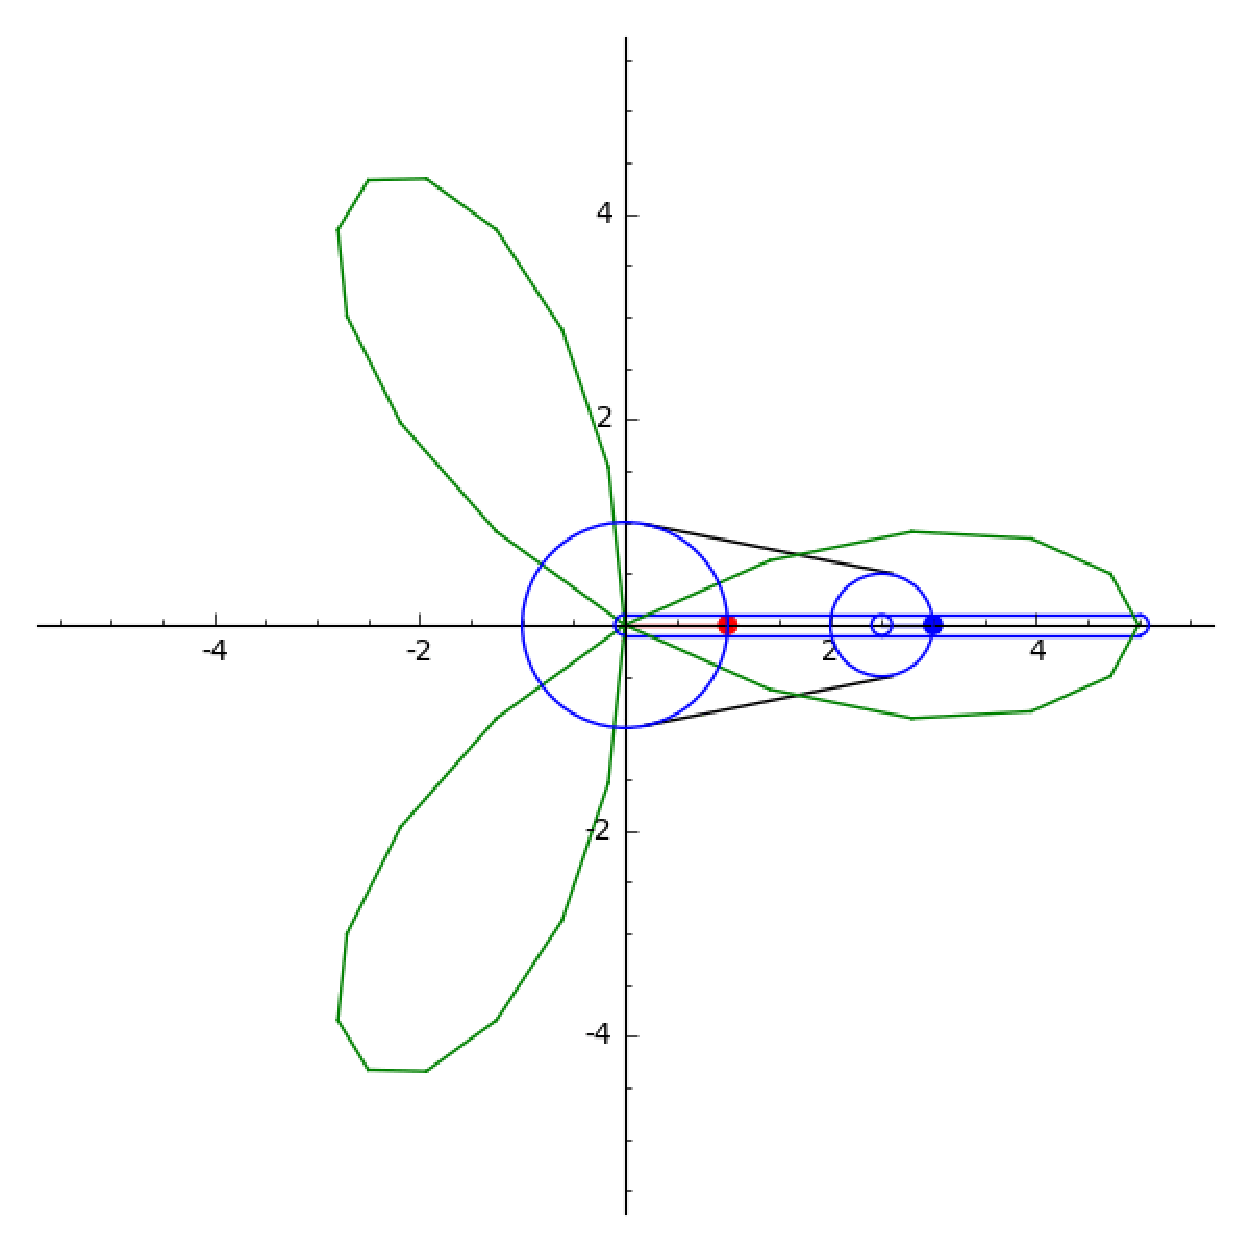
\includegraphics[width=0.25\columnwidth]{tri31.eps}\\[1em]


\end{center}

\end{block}
\end{column}%2


%-- Column 3 ---------------------------------------------------
\begin{column}{0.3\linewidth}

\begin{block}{Trigonometric Plane Curves}
A trigonometric plane curve, is a parameterized curve with coordinate functions that are finite Fourier series, shown as the equation: \\
\begin{equation*}
P =
\left\{\!\begin{aligned}
&x(\theta) \\[1ex]
&y(\theta)
\end{aligned}\right\}
=
\left\{\!\begin{aligned}
&\sum_{k=0}^{m} a_{k} \ cos \  k\theta + b_{k} \ sin  \ k\theta\\[1ex]
&\sum_{k=0}^{m} c_{k}  \ cos \ k\theta + d_{k} \ sin \  k\theta
\end{aligned}\right\}
\end{equation*}

where $a_{k}$, $b_{k}$, $c_{k}$, and $d_{k}$, $k=0,...,m$, are the real coefficients and $\theta \in [0,2\pi]$.

\vspace{2em}
To create the animation in the column to the left, we used the trigonometric plane curve equation for the trifolium:
\[
P_{T}=\begin{cases}
	\hfil -\cos{2\theta} - \cos{4\theta}\\
	\hfil \sin{2\theta} - \sin{4\theta}
	\end{cases}
\]

\end{block}

\begin{block}{Sage}
In order to create the single coupled serial chain that draws our curves, we had to break down its components: two circles, a crank, two chains, two arms, and the curves being drawn. For every frame, our program calculated the position of these components connected to the same input angle $\theta$ and driven by chains at increasing speeds by pulleys of decreasing radius.


\end{block}
%-- Block 4-3
\begin{block}{Conclusions}
The goal of this project was to provide illustrations to mathematical Wikipedia pages that could be better understood through visual applications of its concept. We were able to delve into Kempe's Universality Theorem and understand it through sources used in the article to recreate the mechanisms that draw algebraic curves. Using Sage, we animated a mechanism to draw both the trifolium and hypocycloid curves and post gifs of it to the Wikipedia article to aid future readers.
\end{block}

%-- Block 4-4
\begin{block}{References}
\begin{thebibliography}{99}

\bibitem{design cursive}
Liu Y, Michael McCarthy JJ. Design of a Linkage System to Write in Cursive. ASME. \emph{J. Comput. Inf. Sci. Eng.} 2017;17(3):031015-031015-8. doi:10.1115/1.4037229.

\bibitem{mechanism design}
Liu Y, Michael McCarthy JJ.\emph{ Design of Mechanisms to Draw Trigonometric Plane Curves.} ASME. J. Mechanisms Robotics. 2017;9(2):024503-024503-8. doi:10.1115/1.4035882.  

\bibitem{sage}
SageMath, the Sage Mathematics Software System (Version 7.5.1),
   The Sage Developers, 2017, http://www.sagemath.org.
   
\bibitem{saxena}
Saxena, Anupam. “Kempe's Linkages and the Universality Theorem.” Resonance-Journal of Science Education, vol. 16, no. 3, Mar. 2011, pp. 220–237., www.ias.ac.in/describe/article/reso/016/03/0220-0237.

\bibitem{kempe-wiki}
Wikipedia contributors.\emph{ "Kempe's universality theorem."} Wikipedia, The Free Encyclopedia. Wikipedia, The Free Encyclopedia, 6 Sep. 2017. Web. 25 Oct. 2017.

\bibitem{synthesis of linkage}
Yang Liu, J. Michael McCarthy. \emph{ Synthesis of a linkage to draw a plane algebraic curve} "Mechanism and Machine Theory". Volume 111, 2017, Pages 10-20, ISSN 0094-114X. doi: 10.1016/j.mechmachtheory.2016.12.005.


\end{thebibliography}
\end{block}

\end{column}%3


%-- Column 4 ---------------------------------------------------
%\begin{column}{0.245\linewidth}


%\end{column}%4

\end{columns}
\end{frame}
\end{document}
